% Options for packages loaded elsewhere
\PassOptionsToPackage{unicode}{hyperref}
\PassOptionsToPackage{hyphens}{url}
%
\documentclass[
  12pt,
]{article}
\usepackage{amsmath,amssymb}
\usepackage{setspace}
\usepackage{iftex}
\ifPDFTeX
  \usepackage[T1]{fontenc}
  \usepackage[utf8]{inputenc}
  \usepackage{textcomp} % provide euro and other symbols
\else % if luatex or xetex
  \usepackage{unicode-math} % this also loads fontspec
  \defaultfontfeatures{Scale=MatchLowercase}
  \defaultfontfeatures[\rmfamily]{Ligatures=TeX,Scale=1}
\fi
\usepackage{lmodern}
\ifPDFTeX\else
  % xetex/luatex font selection
    \setmainfont[]{Times New Roman}
    \setmonofont[]{Courier New}
\fi
% Use upquote if available, for straight quotes in verbatim environments
\IfFileExists{upquote.sty}{\usepackage{upquote}}{}
\IfFileExists{microtype.sty}{% use microtype if available
  \usepackage[]{microtype}
  \UseMicrotypeSet[protrusion]{basicmath} % disable protrusion for tt fonts
}{}
\makeatletter
\@ifundefined{KOMAClassName}{% if non-KOMA class
  \IfFileExists{parskip.sty}{%
    \usepackage{parskip}
  }{% else
    \setlength{\parindent}{0pt}
    \setlength{\parskip}{6pt plus 2pt minus 1pt}}
}{% if KOMA class
  \KOMAoptions{parskip=half}}
\makeatother
\usepackage{xcolor}
\usepackage[margin=1in]{geometry}
\usepackage{color}
\usepackage{fancyvrb}
\newcommand{\VerbBar}{|}
\newcommand{\VERB}{\Verb[commandchars=\\\{\}]}
\DefineVerbatimEnvironment{Highlighting}{Verbatim}{commandchars=\\\{\}}
% Add ',fontsize=\small' for more characters per line
\usepackage{framed}
\definecolor{shadecolor}{RGB}{248,248,248}
\newenvironment{Shaded}{\begin{snugshade}}{\end{snugshade}}
\newcommand{\AlertTok}[1]{\textcolor[rgb]{0.94,0.16,0.16}{#1}}
\newcommand{\AnnotationTok}[1]{\textcolor[rgb]{0.56,0.35,0.01}{\textbf{\textit{#1}}}}
\newcommand{\AttributeTok}[1]{\textcolor[rgb]{0.13,0.29,0.53}{#1}}
\newcommand{\BaseNTok}[1]{\textcolor[rgb]{0.00,0.00,0.81}{#1}}
\newcommand{\BuiltInTok}[1]{#1}
\newcommand{\CharTok}[1]{\textcolor[rgb]{0.31,0.60,0.02}{#1}}
\newcommand{\CommentTok}[1]{\textcolor[rgb]{0.56,0.35,0.01}{\textit{#1}}}
\newcommand{\CommentVarTok}[1]{\textcolor[rgb]{0.56,0.35,0.01}{\textbf{\textit{#1}}}}
\newcommand{\ConstantTok}[1]{\textcolor[rgb]{0.56,0.35,0.01}{#1}}
\newcommand{\ControlFlowTok}[1]{\textcolor[rgb]{0.13,0.29,0.53}{\textbf{#1}}}
\newcommand{\DataTypeTok}[1]{\textcolor[rgb]{0.13,0.29,0.53}{#1}}
\newcommand{\DecValTok}[1]{\textcolor[rgb]{0.00,0.00,0.81}{#1}}
\newcommand{\DocumentationTok}[1]{\textcolor[rgb]{0.56,0.35,0.01}{\textbf{\textit{#1}}}}
\newcommand{\ErrorTok}[1]{\textcolor[rgb]{0.64,0.00,0.00}{\textbf{#1}}}
\newcommand{\ExtensionTok}[1]{#1}
\newcommand{\FloatTok}[1]{\textcolor[rgb]{0.00,0.00,0.81}{#1}}
\newcommand{\FunctionTok}[1]{\textcolor[rgb]{0.13,0.29,0.53}{\textbf{#1}}}
\newcommand{\ImportTok}[1]{#1}
\newcommand{\InformationTok}[1]{\textcolor[rgb]{0.56,0.35,0.01}{\textbf{\textit{#1}}}}
\newcommand{\KeywordTok}[1]{\textcolor[rgb]{0.13,0.29,0.53}{\textbf{#1}}}
\newcommand{\NormalTok}[1]{#1}
\newcommand{\OperatorTok}[1]{\textcolor[rgb]{0.81,0.36,0.00}{\textbf{#1}}}
\newcommand{\OtherTok}[1]{\textcolor[rgb]{0.56,0.35,0.01}{#1}}
\newcommand{\PreprocessorTok}[1]{\textcolor[rgb]{0.56,0.35,0.01}{\textit{#1}}}
\newcommand{\RegionMarkerTok}[1]{#1}
\newcommand{\SpecialCharTok}[1]{\textcolor[rgb]{0.81,0.36,0.00}{\textbf{#1}}}
\newcommand{\SpecialStringTok}[1]{\textcolor[rgb]{0.31,0.60,0.02}{#1}}
\newcommand{\StringTok}[1]{\textcolor[rgb]{0.31,0.60,0.02}{#1}}
\newcommand{\VariableTok}[1]{\textcolor[rgb]{0.00,0.00,0.00}{#1}}
\newcommand{\VerbatimStringTok}[1]{\textcolor[rgb]{0.31,0.60,0.02}{#1}}
\newcommand{\WarningTok}[1]{\textcolor[rgb]{0.56,0.35,0.01}{\textbf{\textit{#1}}}}
\usepackage{graphicx}
\makeatletter
\def\maxwidth{\ifdim\Gin@nat@width>\linewidth\linewidth\else\Gin@nat@width\fi}
\def\maxheight{\ifdim\Gin@nat@height>\textheight\textheight\else\Gin@nat@height\fi}
\makeatother
% Scale images if necessary, so that they will not overflow the page
% margins by default, and it is still possible to overwrite the defaults
% using explicit options in \includegraphics[width, height, ...]{}
\setkeys{Gin}{width=\maxwidth,height=\maxheight,keepaspectratio}
% Set default figure placement to htbp
\makeatletter
\def\fps@figure{htbp}
\makeatother
\setlength{\emergencystretch}{3em} % prevent overfull lines
\providecommand{\tightlist}{%
  \setlength{\itemsep}{0pt}\setlength{\parskip}{0pt}}
\setcounter{secnumdepth}{-\maxdimen} % remove section numbering
\usepackage{setspace}
\usepackage{fontspec}
\setmainfont{Times New Roman}
\linespread{2}
\ifLuaTeX
  \usepackage{selnolig}  % disable illegal ligatures
\fi
\usepackage{bookmark}
\IfFileExists{xurl.sty}{\usepackage{xurl}}{} % add URL line breaks if available
\urlstyle{same}
\hypersetup{
  pdftitle={Arkesh Das CMSE 410 Semester Project},
  pdfauthor={Arkesh Das},
  hidelinks,
  pdfcreator={LaTeX via pandoc}}

\title{Arkesh Das CMSE 410 Semester Project}
\author{Arkesh Das}
\date{03/30/2025}

\begin{document}
\maketitle

\setstretch{2}
\section{Assessing the Influence of False Discovery Rate Methods on
Genetic Associations in an Immune Response
GWAS}\label{assessing-the-influence-of-false-discovery-rate-methods-on-genetic-associations-in-an-immune-response-gwas}

\subsection{Background}\label{background}

Genome-wide association studies (GWAS) have emerged as powerful tools
for linking genetic variants with complex traits, including immune
responses. A typical GWAS involves testing millions of single nucleotide
polymorphisms (SNPs) for associations, which leads to a substantial
multiple testing burden. Applying a simple p-value threshold (e.g.,
0.05) is inadequate, as it would generate many false positives. Thus,
false discovery rate (FDR) control has become an essential strategy to
address this challenge.

\subsection{About the data}\label{about-the-data}

This project utilizes data from the Milieu Intérieur (MI) project, a
comprehensive, population-based study coordinated by Prof.~Lluis
Quintana-Murci and Dr.~Darragh Duffy at Institut Pasteur in Paris.
Established under the French Government's Investissement d'Avenir --
Laboratoire d'Excellence (LabEx) initiative, the MI project aims to
dissect the interplay between genetics, environment, and immune
variation {[}1{]}.

It was designed to address a critical discrepancy in medicine: while
immune responses vary widely among individuals, medical care and
therapeutic strategies are often standardized across populations.

I chose to use this dataset because it offers a unique opportunity to
evaluate the impact of false discovery rate methods on GWAS results in
the context of immune variation, and the data is high-resolution and
well-characterized so it's ideal for benchmarking statistical methods.

The data was accessed from the NHGRI-EBI GWAS Catalog. The Catalog is a
publicly available repository of SNP-trait associations identified in
published GWAS studies. It provides standardized annotations, p-values,
effect sizes, and sample information for millions of SNPs across
hundreds of phenotypes.

The MI cohort consists of 1,000 healthy individuals, age- and
sex-stratified across five decades (ages 20--70), and of french origin.
Detailed serological data were collected, including total levels of IgA,
IgE, IgG, and IgM, along with antibody responses to 15 antigens from
common infectious agents and vaccines (e.g., influenza, EBV, CMV, HSV,
rubella). The cohort was genotyped for over 700,000 SNPs and
subsequently imputed to yield over 12 million genetic variants.
Extensive phenotypic, demographic, clinical, and environmental metadata
are also available, including vaccine history, infection exposure, CRP
levels, lipid profiles, and lifestyle factors {[}2{]}.

\section{Loading in the Data}\label{loading-in-the-data}

\section{Reading in the Data and making
dataframes}\label{reading-in-the-data-and-making-dataframes}

\begin{Shaded}
\begin{Highlighting}[]
\CommentTok{\#df will contain all of the data from the study that had MAF \textgreater{} 5\%}
\CommentTok{\#df2 is 1,000 snps, used to test code chunks before running on larger data frames}
\CommentTok{\#df3 contains 100,000 random snps, used as an analogue for the entire data set}
\CommentTok{\#ch6 contains the 354095 snps identified on chromosome 6}

\CommentTok{\#reloading the \textquotesingle{}df\textquotesingle{} dataframe takes a long time because of the number of observations }
\NormalTok{df }\OtherTok{\textless{}{-}} \FunctionTok{read.table}\NormalTok{(}\StringTok{"/Users/arkeshdas/Documents/CMSE 410/repos/HBV\_HBc\_GWAS\_serostatus.txt"}\NormalTok{, }\AttributeTok{header =} \ConstantTok{FALSE}\NormalTok{, }\AttributeTok{sep =} \StringTok{""}\NormalTok{, }\AttributeTok{stringsAsFactors =} \ConstantTok{FALSE}\NormalTok{)}
\FunctionTok{colnames}\NormalTok{(df) }\OtherTok{\textless{}{-}} \FunctionTok{c}\NormalTok{(}\StringTok{"\#CHROM"}\NormalTok{, }\StringTok{"POS"}\NormalTok{, }\StringTok{"ID"}\NormalTok{, }\StringTok{"REF"}\NormalTok{, }\StringTok{"ALT"}\NormalTok{, }\StringTok{"ALT\_FREQ"}\NormalTok{, }\StringTok{"TEST"}\NormalTok{, }\StringTok{"OBS\_CT"}\NormalTok{, }\StringTok{"OR"}\NormalTok{, }\StringTok{"SE"}\NormalTok{, }\StringTok{"T\_STAT"}\NormalTok{, }\StringTok{"P"}\NormalTok{)}
\FunctionTok{head}\NormalTok{(df)}
\end{Highlighting}
\end{Shaded}

\begin{verbatim}
##   #CHROM    POS          ID REF ALT ALT_FREQ TEST OBS_CT      OR       SE
## 1      1 729679   rs4951859   G   C 0.153770  ADD    504 1.85558 0.484720
## 2      1 731718 rs142557973   T   C 0.111111  ADD    504 1.60082 0.535842
## 3      1 734349 rs141242758   T   C 0.107143  ADD    504 1.69814 0.544585
## 4      1 736289  rs79010578   T   A 0.125000  ADD    504 1.47914 0.551837
## 5      1 752566   rs3094315   A   G 0.143849  ADD    504 2.22132 0.453686
## 6      1 752721   rs3131972   G   A 0.143849  ADD    504 2.22132 0.453686
##     T_STAT         P
## 1 1.275370 0.2021780
## 2 0.878092 0.3798940
## 3 0.972362 0.3308700
## 4 0.709382 0.4780870
## 5 1.759150 0.0785516
## 6 1.759150 0.0785516
\end{verbatim}

\begin{Shaded}
\begin{Highlighting}[]
\NormalTok{df2 }\OtherTok{\textless{}{-}} \FunctionTok{read.table}\NormalTok{(}\StringTok{"/Users/arkeshdas/Documents/CMSE 410/repos/HBV\_HBc\_GWAS\_serostatus.txt"}\NormalTok{, }\AttributeTok{header =} \ConstantTok{FALSE}\NormalTok{, }\AttributeTok{sep =} \StringTok{""}\NormalTok{, }\AttributeTok{stringsAsFactors =} \ConstantTok{FALSE}\NormalTok{, }\AttributeTok{nrows =} \DecValTok{1000}\NormalTok{)}
\FunctionTok{colnames}\NormalTok{(df2) }\OtherTok{\textless{}{-}} \FunctionTok{c}\NormalTok{(}\StringTok{"\#CHROM"}\NormalTok{, }\StringTok{"POS"}\NormalTok{, }\StringTok{"ID"}\NormalTok{, }\StringTok{"REF"}\NormalTok{, }\StringTok{"ALT"}\NormalTok{, }\StringTok{"ALT\_FREQ"}\NormalTok{, }\StringTok{"TEST"}\NormalTok{, }\StringTok{"OBS\_CT"}\NormalTok{, }\StringTok{"OR"}\NormalTok{, }\StringTok{"SE"}\NormalTok{, }\StringTok{"T\_STAT"}\NormalTok{, }\StringTok{"P"}\NormalTok{)}
\FunctionTok{head}\NormalTok{(df2)}
\end{Highlighting}
\end{Shaded}

\begin{verbatim}
##   #CHROM    POS          ID REF ALT ALT_FREQ TEST OBS_CT      OR       SE
## 1      1 729679   rs4951859   G   C 0.153770  ADD    504 1.85558 0.484720
## 2      1 731718 rs142557973   T   C 0.111111  ADD    504 1.60082 0.535842
## 3      1 734349 rs141242758   T   C 0.107143  ADD    504 1.69814 0.544585
## 4      1 736289  rs79010578   T   A 0.125000  ADD    504 1.47914 0.551837
## 5      1 752566   rs3094315   A   G 0.143849  ADD    504 2.22132 0.453686
## 6      1 752721   rs3131972   G   A 0.143849  ADD    504 2.22132 0.453686
##     T_STAT         P
## 1 1.275370 0.2021780
## 2 0.878092 0.3798940
## 3 0.972362 0.3308700
## 4 0.709382 0.4780870
## 5 1.759150 0.0785516
## 6 1.759150 0.0785516
\end{verbatim}

\begin{Shaded}
\begin{Highlighting}[]
\FunctionTok{set.seed}\NormalTok{(}\DecValTok{03302025}\NormalTok{)  }\CommentTok{\# Setting seed for reproducibility for df3}
\NormalTok{df3 }\OtherTok{\textless{}{-}}\NormalTok{ df[}\FunctionTok{sample}\NormalTok{(}\FunctionTok{nrow}\NormalTok{(df), }\DecValTok{100000}\NormalTok{), ]}
\FunctionTok{colnames}\NormalTok{(df3) }\OtherTok{\textless{}{-}} \FunctionTok{c}\NormalTok{(}\StringTok{"\#CHROM"}\NormalTok{, }\StringTok{"POS"}\NormalTok{, }\StringTok{"ID"}\NormalTok{, }\StringTok{"REF"}\NormalTok{, }\StringTok{"ALT"}\NormalTok{, }\StringTok{"ALT\_FREQ"}\NormalTok{, }\StringTok{"TEST"}\NormalTok{, }\StringTok{"OBS\_CT"}\NormalTok{, }\StringTok{"OR"}\NormalTok{, }\StringTok{"SE"}\NormalTok{, }\StringTok{"T\_STAT"}\NormalTok{, }\StringTok{"P"}\NormalTok{)}
\FunctionTok{head}\NormalTok{(df3)}
\end{Highlighting}
\end{Shaded}

\begin{verbatim}
##         #CHROM       POS         ID REF ALT  ALT_FREQ TEST OBS_CT       OR
## 5133272     20  58001534  rs6123895   G   A 0.0843254  ADD    504 0.515262
## 2864968      8 123959201 rs35276815   A   G 0.0496032  ADD    504 0.609257
## 2891050      8 135594129 rs72719766   G   A 0.2023810  ADD    504 1.117420
## 4067132     13  82262514  rs9531236   T   C 0.4017860  ADD    504 1.221140
## 1960339      6   3294824  rs9378357   G   T 0.0783730  ADD    504 0.846474
## 3732300     12  24216722  rs7964057   A   G 0.2896830  ADD    504 1.328880
##               SE    T_STAT        P
## 5133272 1.002900 -0.661160 0.508510
## 2864968 1.067520 -0.464174 0.642523
## 2891050 0.449246  0.247121 0.804815
## 4067132 0.415559  0.480766 0.630683
## 1960339 0.771480 -0.216047 0.828951
## 3732300 0.386534  0.735603 0.461973
\end{verbatim}

\begin{Shaded}
\begin{Highlighting}[]
\NormalTok{ch6 }\OtherTok{\textless{}{-}}\NormalTok{ df }\SpecialCharTok{\%\textgreater{}\%} \FunctionTok{filter}\NormalTok{(}\StringTok{\textasciigrave{}}\AttributeTok{\#CHROM}\StringTok{\textasciigrave{}} \SpecialCharTok{==} \DecValTok{6}\NormalTok{)}

\FunctionTok{colnames}\NormalTok{(ch6) }\OtherTok{\textless{}{-}} \FunctionTok{c}\NormalTok{(}\StringTok{"\#CHROM"}\NormalTok{, }\StringTok{"POS"}\NormalTok{, }\StringTok{"ID"}\NormalTok{, }\StringTok{"REF"}\NormalTok{, }\StringTok{"ALT"}\NormalTok{, }\StringTok{"ALT\_FREQ"}\NormalTok{, }\StringTok{"TEST"}\NormalTok{, }\StringTok{"OBS\_CT"}\NormalTok{, }\StringTok{"OR"}\NormalTok{, }\StringTok{"SE"}\NormalTok{, }\StringTok{"T\_STAT"}\NormalTok{, }\StringTok{"P"}\NormalTok{)}
\FunctionTok{head}\NormalTok{(ch6)}
\end{Highlighting}
\end{Shaded}

\begin{verbatim}
##   #CHROM    POS          ID REF ALT  ALT_FREQ TEST OBS_CT       OR       SE
## 1      6 190248 rs115458869   A   G 0.1736110  ADD    504 1.053850 0.506894
## 2      6 191736   rs9502903   A   G 0.3988100  ADD    504 1.966050 0.392648
## 3      6 192106  rs12191783   G   A 0.1567460  ADD    504 0.417576 0.748029
## 4      6 192181  rs61430413   A   G 0.0823413  ADD    504 5.636890 0.521984
## 5      6 192243 rs115258892   C   A 0.0734127  ADD    504 6.031840 0.522290
## 6      6 192300   rs6915646   T   G 0.2242060  ADD    504 1.124090 0.441977
##      T_STAT           P
## 1  0.103479 0.917583000
## 2  1.721710 0.085121500
## 3 -1.167450 0.243027000
## 4  3.313000 0.000923018
## 5  3.440720 0.000580171
## 6  0.264669 0.791265000
\end{verbatim}

\begin{Shaded}
\begin{Highlighting}[]
\NormalTok{df\_clean }\OtherTok{\textless{}{-}}\NormalTok{ df }\SpecialCharTok{\%\textgreater{}\%}
  \FunctionTok{filter}\NormalTok{(}\SpecialCharTok{!}\FunctionTok{is.na}\NormalTok{(P))}
\end{Highlighting}
\end{Shaded}

\section{Creating Manhattan Plots}\label{creating-manhattan-plots}

Because I will be making many Manhattan plots, I initially decided to
create a function that I can pass parameters into rather than creating a
Manhattan plot by hand each time.

\begin{Shaded}
\begin{Highlighting}[]
\NormalTok{generate\_manhattan\_plot }\OtherTok{\textless{}{-}} \ControlFlowTok{function}\NormalTok{(df, }
                                    \AttributeTok{chrom\_col =} \StringTok{"\#CHROM"}\NormalTok{, }
                                    \AttributeTok{pos\_col =} \StringTok{"POS"}\NormalTok{, }
                                    \AttributeTok{pval\_col =} \StringTok{"P"}\NormalTok{, }
                                    \AttributeTok{plot\_title =} \StringTok{"Manhattan Plot"}\NormalTok{, }
                                    \AttributeTok{pval\_cutoff =} \FloatTok{0.05}\NormalTok{) \{}

  \CommentTok{\# Step 1: Normalize CHR and BP}
\NormalTok{  df }\OtherTok{\textless{}{-}}\NormalTok{ df }\SpecialCharTok{\%\textgreater{}\%}
    \FunctionTok{mutate}\NormalTok{(}\AttributeTok{CHR =} \FunctionTok{gsub}\NormalTok{(}\StringTok{"chr"}\NormalTok{, }\StringTok{""}\NormalTok{, .data[[chrom\_col]], }\AttributeTok{ignore.case =} \ConstantTok{TRUE}\NormalTok{),}
           \AttributeTok{CHR =} \FunctionTok{gsub}\NormalTok{(}\StringTok{"[\^{}0{-}9XYMT]"}\NormalTok{, }\StringTok{""}\NormalTok{, CHR),}
           \AttributeTok{CHR =} \FunctionTok{as.character}\NormalTok{(CHR),}
           \AttributeTok{BP =} \FunctionTok{as.numeric}\NormalTok{(.data[[pos\_col]])) }\SpecialCharTok{\%\textgreater{}\%}
    \FunctionTok{filter}\NormalTok{(}\SpecialCharTok{!}\FunctionTok{is.na}\NormalTok{(BP) }\SpecialCharTok{\&} \SpecialCharTok{!}\FunctionTok{is.na}\NormalTok{(CHR))}

  \CommentTok{\# Step 2: Sort}
\NormalTok{  df }\OtherTok{\textless{}{-}}\NormalTok{ df }\SpecialCharTok{\%\textgreater{}\%} \FunctionTok{arrange}\NormalTok{(}\FunctionTok{as.numeric}\NormalTok{(CHR), BP)}

  \CommentTok{\# Step 3: Chromosome summary}
\NormalTok{  df\_chr }\OtherTok{\textless{}{-}}\NormalTok{ df }\SpecialCharTok{\%\textgreater{}\%}
    \FunctionTok{group\_by}\NormalTok{(CHR) }\SpecialCharTok{\%\textgreater{}\%}
    \FunctionTok{summarise}\NormalTok{(}\AttributeTok{max\_bp =} \FunctionTok{max}\NormalTok{(BP, }\AttributeTok{na.rm =} \ConstantTok{TRUE}\NormalTok{), }\AttributeTok{.groups =} \StringTok{"drop"}\NormalTok{) }\SpecialCharTok{\%\textgreater{}\%}
    \FunctionTok{arrange}\NormalTok{(}\FunctionTok{as.numeric}\NormalTok{(CHR)) }\SpecialCharTok{\%\textgreater{}\%}
    \FunctionTok{mutate}\NormalTok{(}\AttributeTok{cumulative =} \FunctionTok{cumsum}\NormalTok{(max\_bp) }\SpecialCharTok{{-}}\NormalTok{ max\_bp)}

  \CommentTok{\# Step 4: Merge}
\NormalTok{  df }\OtherTok{\textless{}{-}}\NormalTok{ df }\SpecialCharTok{\%\textgreater{}\%}
    \FunctionTok{left\_join}\NormalTok{(df\_chr, }\AttributeTok{by =} \StringTok{"CHR"}\NormalTok{) }\SpecialCharTok{\%\textgreater{}\%}
    \FunctionTok{filter}\NormalTok{(}\SpecialCharTok{!}\FunctionTok{is.na}\NormalTok{(cumulative)) }\SpecialCharTok{\%\textgreater{}\%}
    \FunctionTok{mutate}\NormalTok{(}\AttributeTok{BP\_cum =}\NormalTok{ BP }\SpecialCharTok{+}\NormalTok{ cumulative)}

  \CommentTok{\# Step 5: Axis labels}
\NormalTok{  axis\_df }\OtherTok{\textless{}{-}}\NormalTok{ df }\SpecialCharTok{\%\textgreater{}\%}
    \FunctionTok{group\_by}\NormalTok{(CHR) }\SpecialCharTok{\%\textgreater{}\%}
    \FunctionTok{summarise}\NormalTok{(}\AttributeTok{center =}\NormalTok{ (}\FunctionTok{min}\NormalTok{(BP\_cum) }\SpecialCharTok{+} \FunctionTok{max}\NormalTok{(BP\_cum)) }\SpecialCharTok{/} \DecValTok{2}\NormalTok{, }\AttributeTok{.groups =} \StringTok{"drop"}\NormalTok{)}

  \CommentTok{\# Step 6: Color map}
\NormalTok{  chroms }\OtherTok{\textless{}{-}} \FunctionTok{sort}\NormalTok{(}\FunctionTok{unique}\NormalTok{(df}\SpecialCharTok{$}\NormalTok{CHR))}
\NormalTok{  chrom\_colors }\OtherTok{\textless{}{-}} \FunctionTok{rep}\NormalTok{(}\FunctionTok{c}\NormalTok{(}\StringTok{"grey"}\NormalTok{, }\StringTok{"skyblue"}\NormalTok{), }\AttributeTok{length.out =} \FunctionTok{length}\NormalTok{(chroms))}
  \FunctionTok{names}\NormalTok{(chrom\_colors) }\OtherTok{\textless{}{-}}\NormalTok{ chroms}

  \CommentTok{\# Step 7: Manhattan Plot}
  \FunctionTok{ggplot}\NormalTok{(df, }\FunctionTok{aes}\NormalTok{(}\AttributeTok{x =}\NormalTok{ BP\_cum, }\AttributeTok{y =} \SpecialCharTok{{-}}\FunctionTok{log10}\NormalTok{(.data[[pval\_col]]))) }\SpecialCharTok{+}
    \FunctionTok{geom\_point}\NormalTok{(}\FunctionTok{aes}\NormalTok{(}\AttributeTok{color =}\NormalTok{ CHR), }\AttributeTok{alpha =} \FloatTok{0.75}\NormalTok{, }\AttributeTok{size =} \FloatTok{1.3}\NormalTok{) }\SpecialCharTok{+}
    \FunctionTok{scale\_color\_manual}\NormalTok{(}\AttributeTok{values =}\NormalTok{ chrom\_colors) }\SpecialCharTok{+}
    \FunctionTok{scale\_x\_continuous}\NormalTok{(}\AttributeTok{label =}\NormalTok{ axis\_df}\SpecialCharTok{$}\NormalTok{CHR, }\AttributeTok{breaks =}\NormalTok{ axis\_df}\SpecialCharTok{$}\NormalTok{center) }\SpecialCharTok{+}
    \FunctionTok{labs}\NormalTok{(}\AttributeTok{x =} \StringTok{"Chromosome"}\NormalTok{, }
         \AttributeTok{y =} \FunctionTok{expression}\NormalTok{(}\SpecialCharTok{{-}}\NormalTok{log[}\DecValTok{10}\NormalTok{](p}\SpecialCharTok{{-}}\NormalTok{value)), }
         \AttributeTok{title =}\NormalTok{ plot\_title) }\SpecialCharTok{+}
    \FunctionTok{geom\_hline}\NormalTok{(}\AttributeTok{yintercept =} \SpecialCharTok{{-}}\FunctionTok{log10}\NormalTok{(pval\_cutoff), }\AttributeTok{linetype =} \StringTok{"dashed"}\NormalTok{, }\AttributeTok{color =} \StringTok{"red"}\NormalTok{) }\SpecialCharTok{+}
    \FunctionTok{theme\_minimal}\NormalTok{() }\SpecialCharTok{+}
    \FunctionTok{theme}\NormalTok{(}\AttributeTok{legend.position =} \StringTok{"none"}\NormalTok{,}
          \AttributeTok{panel.border =} \FunctionTok{element\_blank}\NormalTok{(),}
          \AttributeTok{panel.grid.major.x =} \FunctionTok{element\_blank}\NormalTok{())}
\NormalTok{\}}
\end{Highlighting}
\end{Shaded}

\begin{Shaded}
\begin{Highlighting}[]
\FunctionTok{generate\_manhattan\_plot}\NormalTok{(df3, }\AttributeTok{pval\_cutoff =} \FloatTok{0.05}\NormalTok{, }\AttributeTok{plot\_title =} \StringTok{"Manhattan Plot of Raw P{-}values for 100,000 SNPs"}\NormalTok{)}
\end{Highlighting}
\end{Shaded}

\includegraphics{Arkesh_Das_CMSE_410_Semester_Project_files/figure-latex/testing function-1.pdf}

However, after doing some research, I learned there are already existing
functions that create Manhattan plots (\texttt{qqman} library), so I
will be using this function to create my Manhattan plots instead
{[}3{]}.

\begin{Shaded}
\begin{Highlighting}[]
\NormalTok{df3\_clean }\OtherTok{\textless{}{-}}\NormalTok{ df3 }\SpecialCharTok{\%\textgreater{}\%}
  \FunctionTok{filter}\NormalTok{(}\SpecialCharTok{!}\FunctionTok{is.na}\NormalTok{(P))}
\FunctionTok{manhattan}\NormalTok{(df3\_clean, }\AttributeTok{chr =} \StringTok{"\#CHROM"}\NormalTok{, }\AttributeTok{bp =} \StringTok{"POS"}\NormalTok{, }\AttributeTok{snp =} \StringTok{"ID"}\NormalTok{, }\AttributeTok{p =} \StringTok{"P"}\NormalTok{, }\AttributeTok{suggestiveline =} \ConstantTok{FALSE}\NormalTok{,}
          \AttributeTok{genomewideline =} \SpecialCharTok{{-}}\FunctionTok{log10}\NormalTok{(}\FloatTok{2.7e{-}09}\NormalTok{), }\AttributeTok{ylim =} \FunctionTok{c}\NormalTok{(}\DecValTok{0}\NormalTok{, }\DecValTok{10}\NormalTok{)) }
\FunctionTok{title}\NormalTok{(}\AttributeTok{main =} \StringTok{"Manhattan Plot of Raw P{-}values for 100,000 SNPs Bonferroni"}\NormalTok{)}
\FunctionTok{abline}\NormalTok{(}\AttributeTok{h =} \SpecialCharTok{{-}}\FunctionTok{log10}\NormalTok{(}\FloatTok{9.5e{-}09}\NormalTok{), }\AttributeTok{col =} \StringTok{"darkgreen"}\NormalTok{, }\AttributeTok{lty =} \DecValTok{3}\NormalTok{)}
\end{Highlighting}
\end{Shaded}

\includegraphics{Arkesh_Das_CMSE_410_Semester_Project_files/figure-latex/qqman 100k Bonferroni-1.pdf}

\begin{Shaded}
\begin{Highlighting}[]
\NormalTok{ch6\_clean }\OtherTok{\textless{}{-}}\NormalTok{ ch6 }\SpecialCharTok{\%\textgreater{}\%}
  \FunctionTok{filter}\NormalTok{(}\SpecialCharTok{!}\FunctionTok{is.na}\NormalTok{(P))}
\FunctionTok{manhattan}\NormalTok{(ch6\_clean, }\AttributeTok{chr =} \StringTok{"\#CHROM"}\NormalTok{, }\AttributeTok{bp =} \StringTok{"POS"}\NormalTok{, }\AttributeTok{snp =} \StringTok{"ID"}\NormalTok{, }\AttributeTok{p =} \StringTok{"P"}\NormalTok{, }\AttributeTok{highlight =} \StringTok{"rs4254998"}\NormalTok{,}
          \AttributeTok{genomewideline =} \SpecialCharTok{{-}}\FunctionTok{log10}\NormalTok{(}\FloatTok{0.05}\NormalTok{), }\AttributeTok{ylim =} \FunctionTok{c}\NormalTok{(}\DecValTok{0}\NormalTok{, }\DecValTok{6}\NormalTok{)) }
\FunctionTok{title}\NormalTok{(}\AttributeTok{main =} \StringTok{"Manhattan Plot of Raw P{-}values for Chr. 6 SNPs p = 0.05"}\NormalTok{)}
\end{Highlighting}
\end{Shaded}

\includegraphics{Arkesh_Das_CMSE_410_Semester_Project_files/figure-latex/qqman ch6 0.05-1.pdf}
\# QQ plots

I tried to create my code to create a QQ plot before I realized that
there already is one in \texttt{qqman}

\begin{Shaded}
\begin{Highlighting}[]
\NormalTok{pvals }\OtherTok{\textless{}{-}}\NormalTok{ df3}\SpecialCharTok{$}\NormalTok{P}
\NormalTok{pvals }\OtherTok{\textless{}{-}}\NormalTok{ pvals[}\SpecialCharTok{!}\FunctionTok{is.na}\NormalTok{(pvals)]}

\NormalTok{n }\OtherTok{\textless{}{-}} \FunctionTok{length}\NormalTok{(pvals)}

\NormalTok{expected }\OtherTok{\textless{}{-}} \SpecialCharTok{{-}}\FunctionTok{log10}\NormalTok{(}\FunctionTok{ppoints}\NormalTok{(n))}
\NormalTok{observed }\OtherTok{\textless{}{-}} \SpecialCharTok{{-}}\FunctionTok{log10}\NormalTok{(}\FunctionTok{sort}\NormalTok{(pvals))}

\FunctionTok{plot}\NormalTok{(expected, observed,}
     \AttributeTok{pch =} \DecValTok{19}\NormalTok{,}
     \AttributeTok{col =} \FunctionTok{rgb}\NormalTok{(}\DecValTok{0}\NormalTok{, }\DecValTok{0}\NormalTok{, }\DecValTok{0}\NormalTok{, }\FloatTok{0.5}\NormalTok{),}
     \AttributeTok{cex =} \FloatTok{0.6}\NormalTok{,}
     \AttributeTok{xlab =} \StringTok{"Expected {-}log10(p)"}\NormalTok{,}
     \AttributeTok{ylab =} \StringTok{"Observed {-}log10(p)"}\NormalTok{,}
     \AttributeTok{main =} \StringTok{"QQ Plot of GWAS P{-}values"}\NormalTok{)}

\FunctionTok{abline}\NormalTok{(}\DecValTok{0}\NormalTok{, }\DecValTok{1}\NormalTok{, }\AttributeTok{col =} \StringTok{"red"}\NormalTok{, }\AttributeTok{lwd =} \DecValTok{2}\NormalTok{)}
\end{Highlighting}
\end{Shaded}

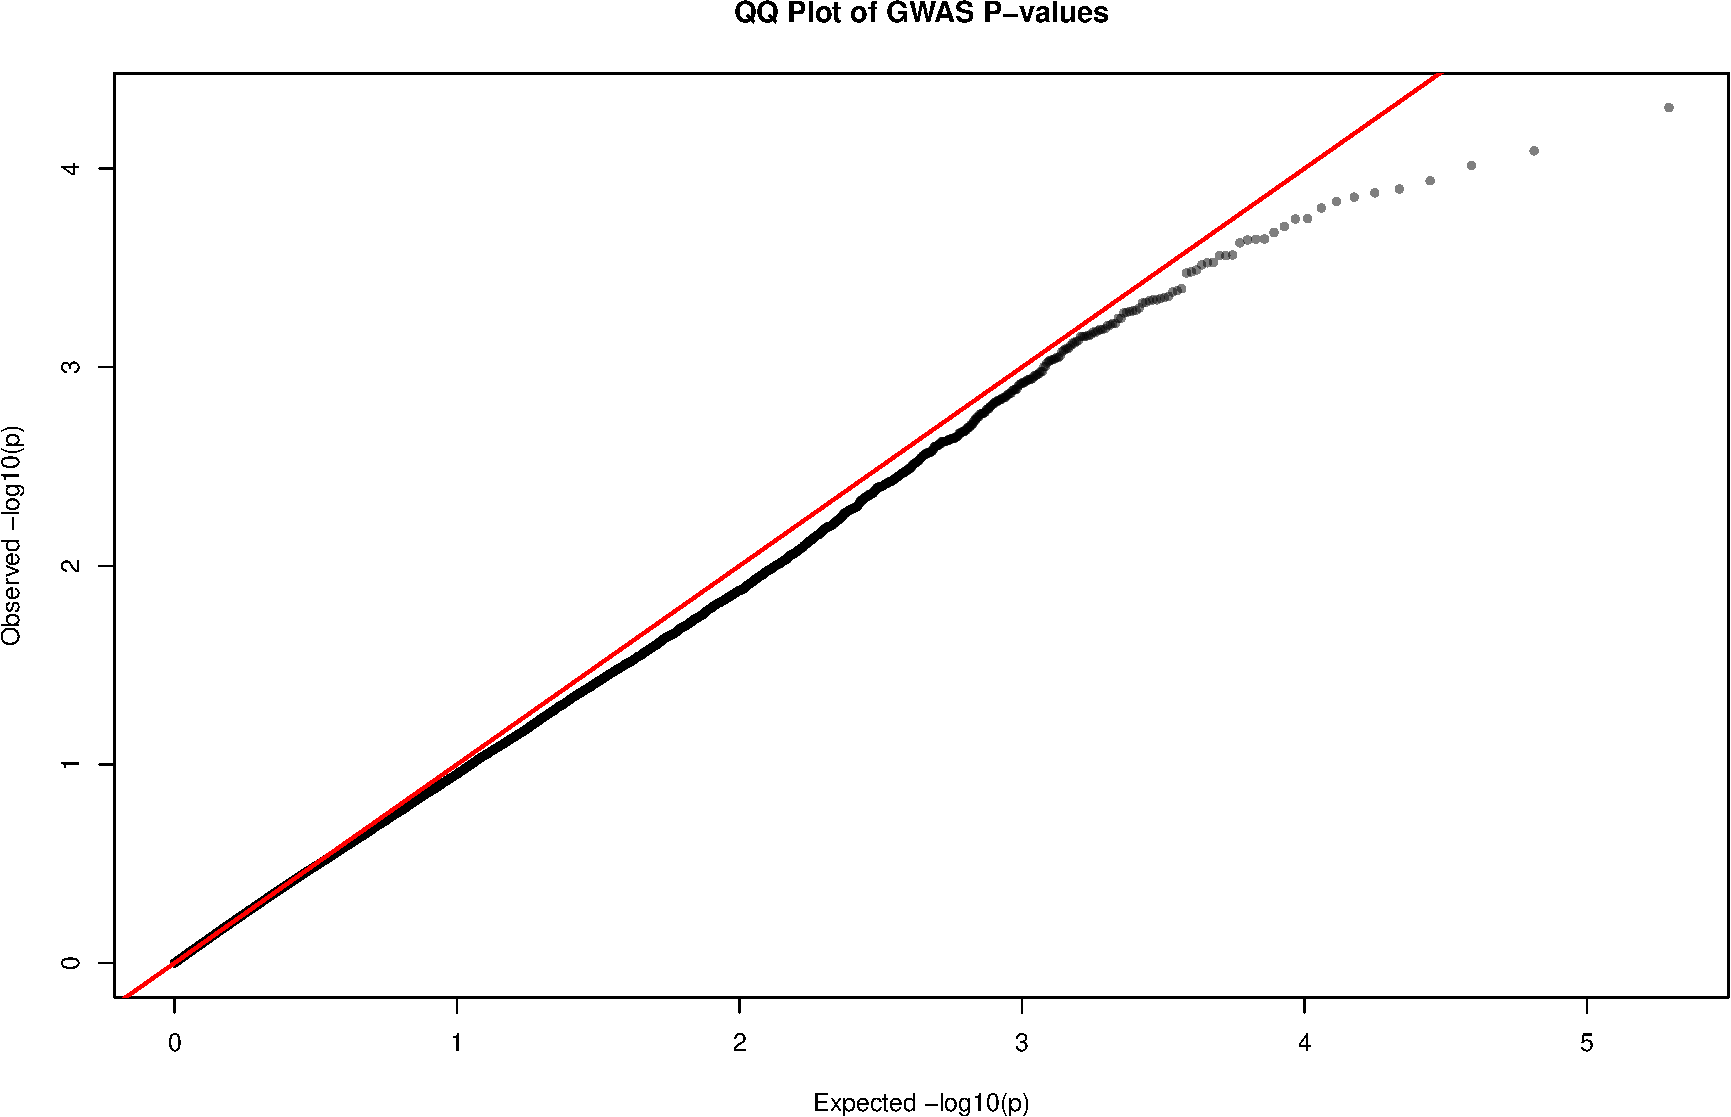
\includegraphics{Arkesh_Das_CMSE_410_Semester_Project_files/figure-latex/QQ plot for subset-1.pdf}

\begin{Shaded}
\begin{Highlighting}[]
\FunctionTok{qq}\NormalTok{(df3\_clean}\SpecialCharTok{$}\NormalTok{P, }\AttributeTok{main =} \StringTok{"QQ Plot of GWAS P{-}values for 100k SNPs"}\NormalTok{)}
\end{Highlighting}
\end{Shaded}

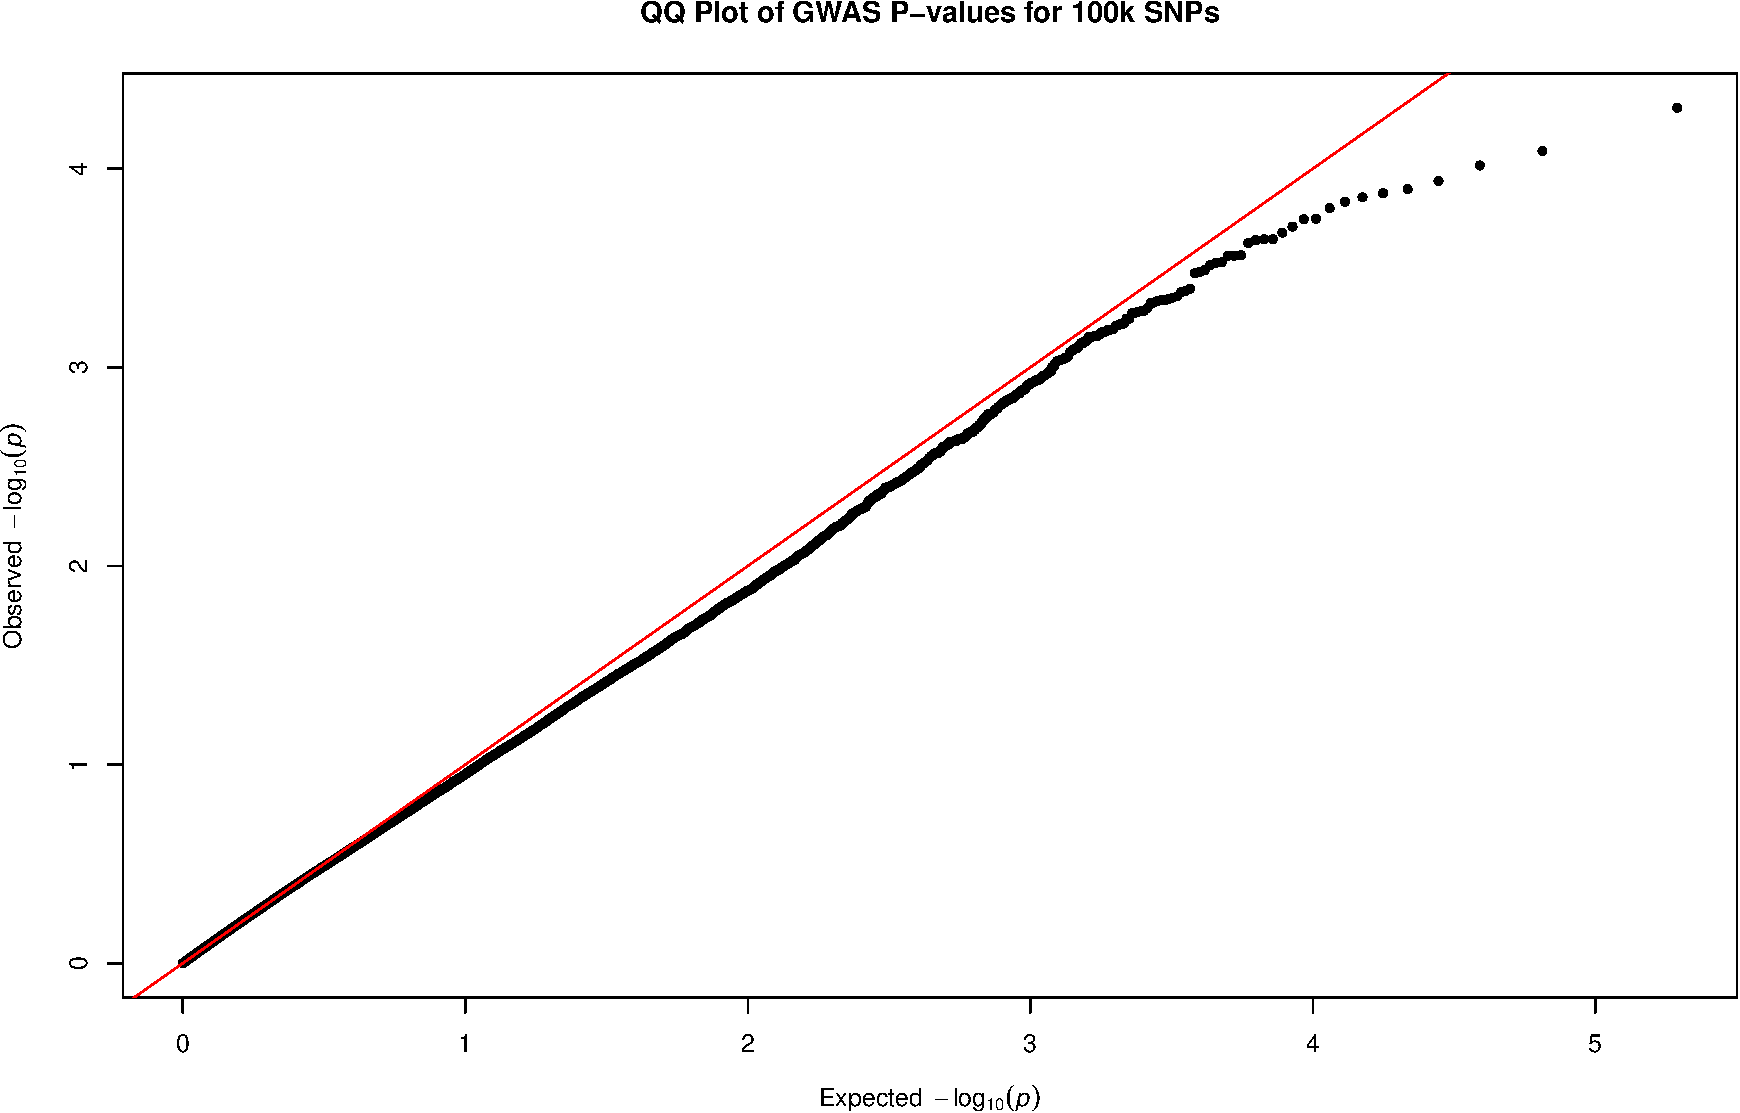
\includegraphics{Arkesh_Das_CMSE_410_Semester_Project_files/figure-latex/qqplot 100k-1.pdf}

\begin{Shaded}
\begin{Highlighting}[]
\FunctionTok{qq}\NormalTok{(ch6\_clean}\SpecialCharTok{$}\NormalTok{P, }\AttributeTok{main =} \StringTok{"QQ Plot of GWAS P{-}values for Chr. 6"}\NormalTok{)}
\end{Highlighting}
\end{Shaded}

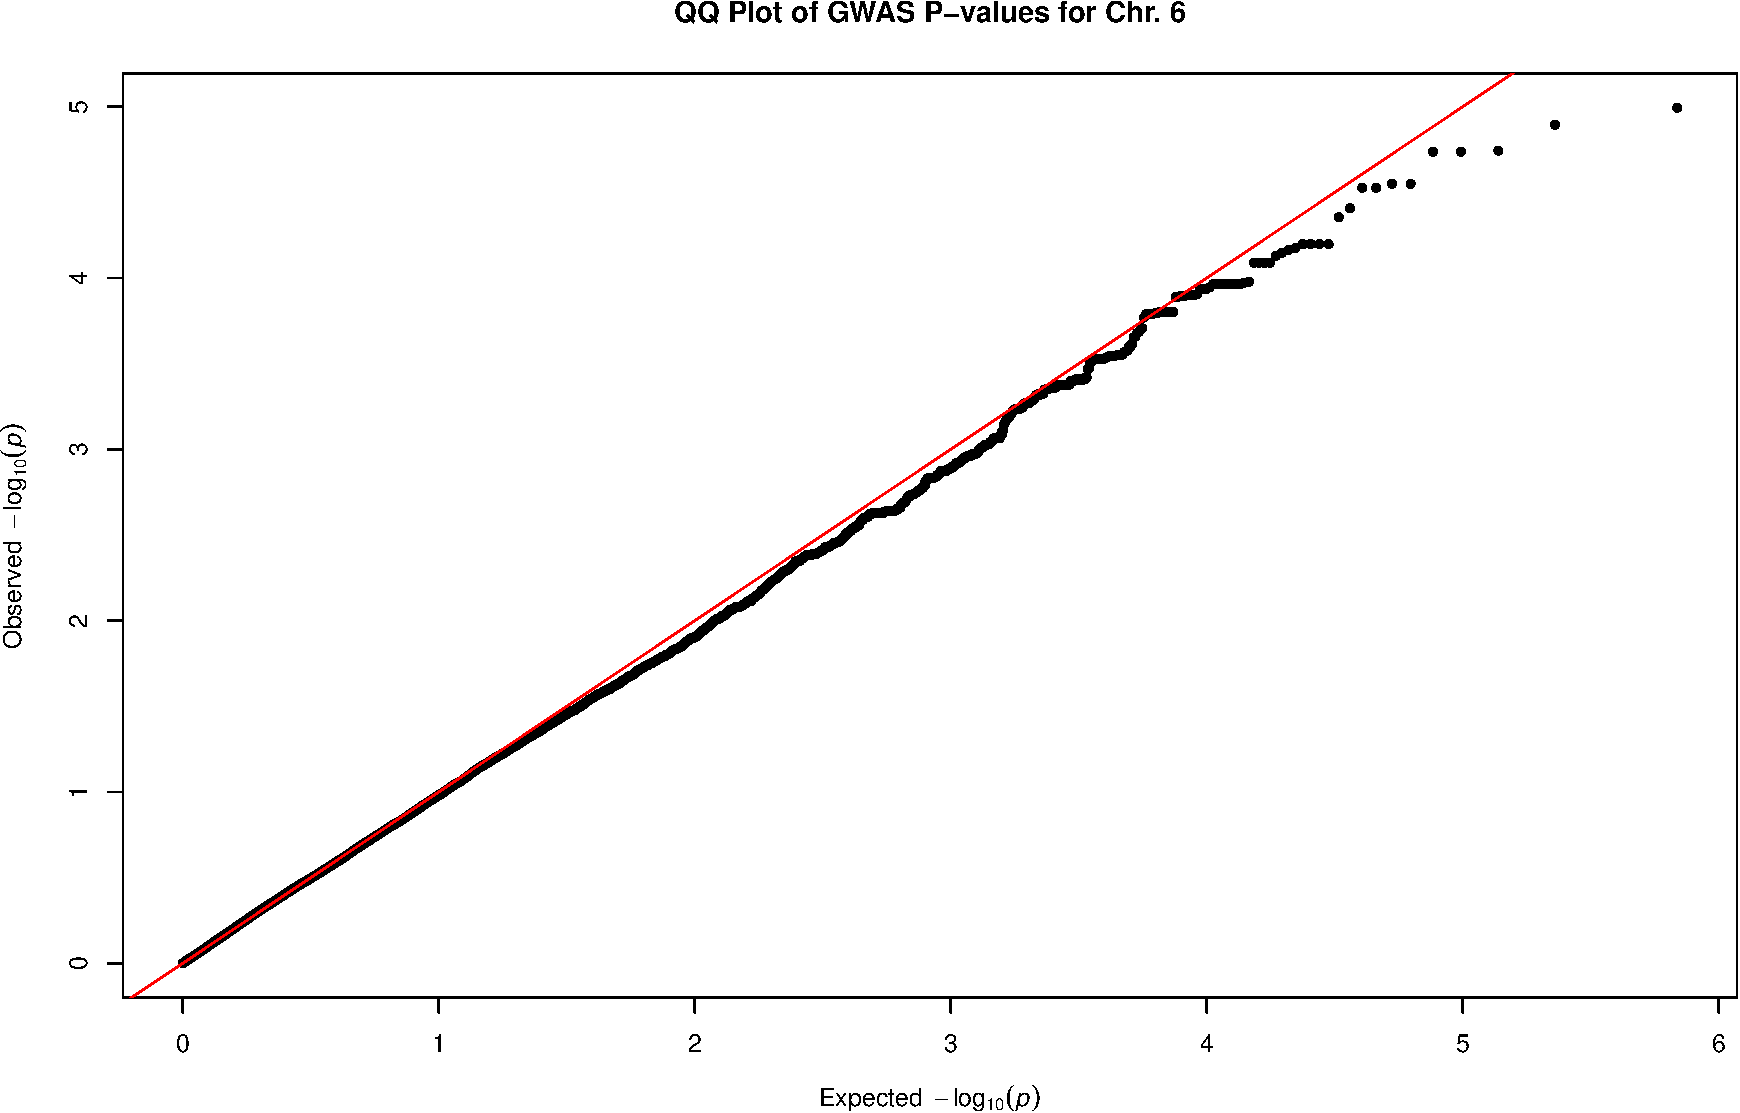
\includegraphics{Arkesh_Das_CMSE_410_Semester_Project_files/figure-latex/qqplot chr6-1.pdf}

\section{Various FDR methods}\label{various-fdr-methods}

Now I will be trying different FDR methods, from most to least
conservative.

\subsection{Benjamini-Yekutieli}\label{benjamini-yekutieli}

Out of the p-value adjustment methods, Benjamini Yekuteli is the most
conservative, so I will try it first. R has a \texttt{p.adjust} function
that can automatically apply the BY method.

\begin{Shaded}
\begin{Highlighting}[]
\NormalTok{df3\_clean}\SpecialCharTok{$}\NormalTok{P\_BY }\OtherTok{\textless{}{-}} \FunctionTok{p.adjust}\NormalTok{(df3\_clean}\SpecialCharTok{$}\NormalTok{P, }\AttributeTok{method =} \StringTok{"BY"}\NormalTok{)}

\CommentTok{\# Summary stats of BY{-}adjusted p{-}values}
\FunctionTok{summary}\NormalTok{(df3\_clean}\SpecialCharTok{$}\NormalTok{P\_BY)}
\end{Highlighting}
\end{Shaded}

\begin{verbatim}
##    Min. 1st Qu.  Median    Mean 3rd Qu.    Max. 
##       1       1       1       1       1       1
\end{verbatim}

\begin{Shaded}
\begin{Highlighting}[]
\CommentTok{\# Filter significant results under BY }
\NormalTok{df3\_by\_sig }\OtherTok{\textless{}{-}}\NormalTok{ df3\_clean }\SpecialCharTok{\%\textgreater{}\%} \FunctionTok{filter}\NormalTok{(P\_BY }\SpecialCharTok{\textless{}} \FloatTok{0.05}\NormalTok{)}

\FunctionTok{manhattan}\NormalTok{(df3\_clean, }\AttributeTok{chr =} \StringTok{"\#CHROM"}\NormalTok{, }\AttributeTok{bp =} \StringTok{"POS"}\NormalTok{, }\AttributeTok{snp =} \StringTok{"ID"}\NormalTok{, }\AttributeTok{p =} \StringTok{"P\_BY"}\NormalTok{, }\AttributeTok{suggestiveline =} \ConstantTok{FALSE}\NormalTok{, }\AttributeTok{ylim =} \FunctionTok{c}\NormalTok{(}\DecValTok{0}\NormalTok{,}\DecValTok{1}\NormalTok{)) }
\FunctionTok{title}\NormalTok{(}\AttributeTok{main =} \StringTok{"Manhattan Plot of BY adjusted P{-}values for 100,000 SNPs"}\NormalTok{)}
\end{Highlighting}
\end{Shaded}

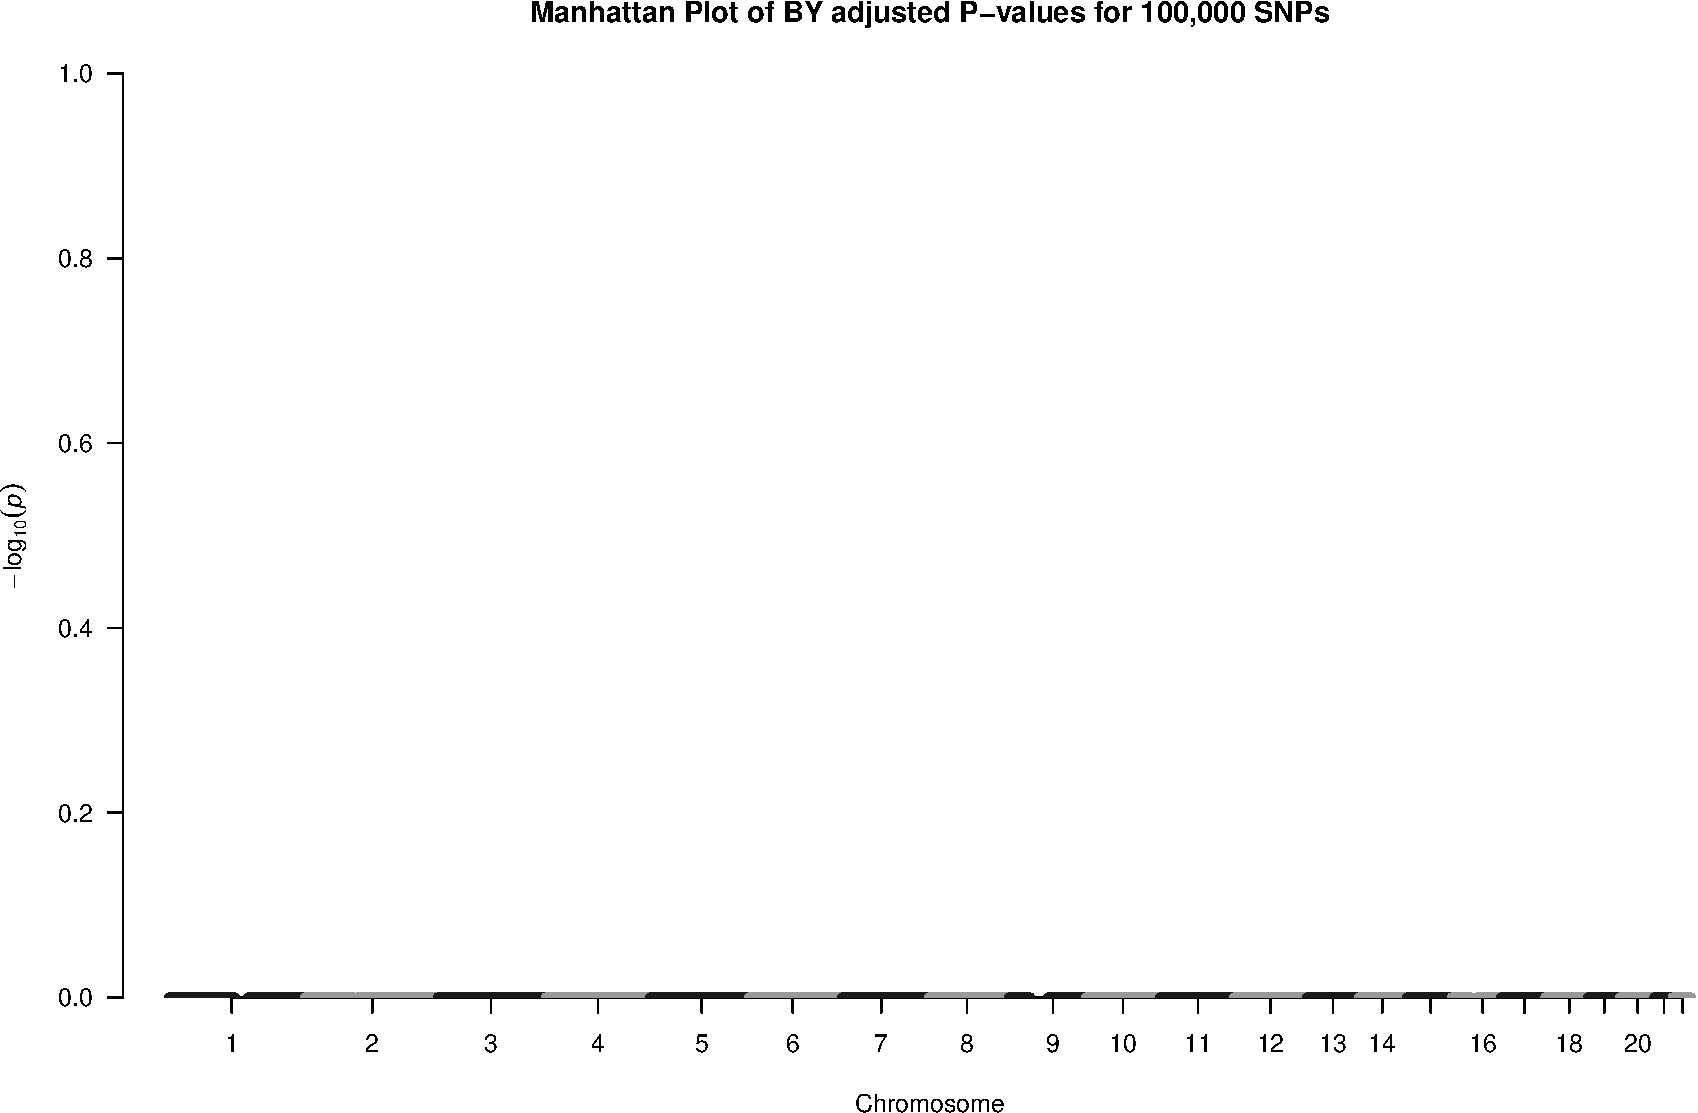
\includegraphics{Arkesh_Das_CMSE_410_Semester_Project_files/figure-latex/Benjamini-Yekutieli test-1.pdf}

I cannot visualize the BY-adjusted p-values using my Manhattan Plot. In
this case, I can thankfully modify and re-use my plotting function from
earlier:

\begin{Shaded}
\begin{Highlighting}[]
\NormalTok{generate\_plot }\OtherTok{\textless{}{-}} \ControlFlowTok{function}\NormalTok{(df, }
                                    \AttributeTok{chrom\_col =} \StringTok{"\#CHROM"}\NormalTok{, }
                                    \AttributeTok{pos\_col =} \StringTok{"POS"}\NormalTok{, }
                                    \AttributeTok{pval\_col =} \StringTok{"P"}\NormalTok{, }
                                    \AttributeTok{plot\_title =} \StringTok{"Plot"}\NormalTok{) \{}

  \CommentTok{\# Step 1: Normalize CHR and BP}
\NormalTok{  df }\OtherTok{\textless{}{-}}\NormalTok{ df }\SpecialCharTok{\%\textgreater{}\%}
    \FunctionTok{mutate}\NormalTok{(}\AttributeTok{CHR =} \FunctionTok{gsub}\NormalTok{(}\StringTok{"chr"}\NormalTok{, }\StringTok{""}\NormalTok{, .data[[chrom\_col]], }\AttributeTok{ignore.case =} \ConstantTok{TRUE}\NormalTok{),}
           \AttributeTok{CHR =} \FunctionTok{gsub}\NormalTok{(}\StringTok{"[\^{}0{-}9XYMT]"}\NormalTok{, }\StringTok{""}\NormalTok{, CHR),}
           \AttributeTok{CHR =} \FunctionTok{as.character}\NormalTok{(CHR),}
           \AttributeTok{BP =} \FunctionTok{as.numeric}\NormalTok{(.data[[pos\_col]])) }\SpecialCharTok{\%\textgreater{}\%}
    \FunctionTok{filter}\NormalTok{(}\SpecialCharTok{!}\FunctionTok{is.na}\NormalTok{(BP) }\SpecialCharTok{\&} \SpecialCharTok{!}\FunctionTok{is.na}\NormalTok{(CHR))}

  \CommentTok{\# Step 2: Sort}
\NormalTok{  df }\OtherTok{\textless{}{-}}\NormalTok{ df }\SpecialCharTok{\%\textgreater{}\%} \FunctionTok{arrange}\NormalTok{(}\FunctionTok{as.numeric}\NormalTok{(CHR), BP)}

  \CommentTok{\# Step 3: Chromosome summary}
\NormalTok{  df\_chr }\OtherTok{\textless{}{-}}\NormalTok{ df }\SpecialCharTok{\%\textgreater{}\%}
    \FunctionTok{group\_by}\NormalTok{(CHR) }\SpecialCharTok{\%\textgreater{}\%}
    \FunctionTok{summarise}\NormalTok{(}\AttributeTok{max\_bp =} \FunctionTok{max}\NormalTok{(BP, }\AttributeTok{na.rm =} \ConstantTok{TRUE}\NormalTok{), }\AttributeTok{.groups =} \StringTok{"drop"}\NormalTok{) }\SpecialCharTok{\%\textgreater{}\%}
    \FunctionTok{arrange}\NormalTok{(}\FunctionTok{as.numeric}\NormalTok{(CHR)) }\SpecialCharTok{\%\textgreater{}\%}
    \FunctionTok{mutate}\NormalTok{(}\AttributeTok{cumulative =} \FunctionTok{cumsum}\NormalTok{(max\_bp) }\SpecialCharTok{{-}}\NormalTok{ max\_bp)}

  \CommentTok{\# Step 4: Merge}
\NormalTok{  df }\OtherTok{\textless{}{-}}\NormalTok{ df }\SpecialCharTok{\%\textgreater{}\%}
    \FunctionTok{left\_join}\NormalTok{(df\_chr, }\AttributeTok{by =} \StringTok{"CHR"}\NormalTok{) }\SpecialCharTok{\%\textgreater{}\%}
    \FunctionTok{filter}\NormalTok{(}\SpecialCharTok{!}\FunctionTok{is.na}\NormalTok{(cumulative)) }\SpecialCharTok{\%\textgreater{}\%}
    \FunctionTok{mutate}\NormalTok{(}\AttributeTok{BP\_cum =}\NormalTok{ BP }\SpecialCharTok{+}\NormalTok{ cumulative)}

  \CommentTok{\# Step 5: Axis labels}
\NormalTok{  axis\_df }\OtherTok{\textless{}{-}}\NormalTok{ df }\SpecialCharTok{\%\textgreater{}\%}
    \FunctionTok{group\_by}\NormalTok{(CHR) }\SpecialCharTok{\%\textgreater{}\%}
    \FunctionTok{summarise}\NormalTok{(}\AttributeTok{center =}\NormalTok{ (}\FunctionTok{min}\NormalTok{(BP\_cum) }\SpecialCharTok{+} \FunctionTok{max}\NormalTok{(BP\_cum)) }\SpecialCharTok{/} \DecValTok{2}\NormalTok{, }\AttributeTok{.groups =} \StringTok{"drop"}\NormalTok{)}

  \CommentTok{\# Step 6: Color map}
\NormalTok{  chroms }\OtherTok{\textless{}{-}} \FunctionTok{sort}\NormalTok{(}\FunctionTok{unique}\NormalTok{(df}\SpecialCharTok{$}\NormalTok{CHR))}
\NormalTok{  chrom\_colors }\OtherTok{\textless{}{-}} \FunctionTok{rep}\NormalTok{(}\FunctionTok{c}\NormalTok{(}\StringTok{"grey"}\NormalTok{, }\StringTok{"skyblue"}\NormalTok{), }\AttributeTok{length.out =} \FunctionTok{length}\NormalTok{(chroms))}
  \FunctionTok{names}\NormalTok{(chrom\_colors) }\OtherTok{\textless{}{-}}\NormalTok{ chroms}

  \CommentTok{\# Step 7: Plot}
  \FunctionTok{ggplot}\NormalTok{(df, }\FunctionTok{aes}\NormalTok{(}\AttributeTok{x =}\NormalTok{ BP\_cum, }\AttributeTok{y =}\NormalTok{ .data[[pval\_col]])) }\SpecialCharTok{+}
    \FunctionTok{geom\_point}\NormalTok{(}\FunctionTok{aes}\NormalTok{(}\AttributeTok{color =}\NormalTok{ CHR), }\AttributeTok{alpha =} \FloatTok{0.75}\NormalTok{, }\AttributeTok{size =} \FloatTok{1.3}\NormalTok{) }\SpecialCharTok{+}
    \FunctionTok{scale\_color\_manual}\NormalTok{(}\AttributeTok{values =}\NormalTok{ chrom\_colors) }\SpecialCharTok{+}
    \FunctionTok{scale\_x\_continuous}\NormalTok{(}\AttributeTok{label =}\NormalTok{ axis\_df}\SpecialCharTok{$}\NormalTok{CHR, }\AttributeTok{breaks =}\NormalTok{ axis\_df}\SpecialCharTok{$}\NormalTok{center) }\SpecialCharTok{+}
    \FunctionTok{ylim}\NormalTok{(}\DecValTok{0}\NormalTok{,}\FloatTok{0.007}\NormalTok{)}\SpecialCharTok{+}
    \FunctionTok{labs}\NormalTok{(}\AttributeTok{x =} \StringTok{"Chromosome"}\NormalTok{, }
         \AttributeTok{y =} \StringTok{\textquotesingle{}p{-}value\textquotesingle{}}\NormalTok{, }
         \AttributeTok{title =}\NormalTok{ plot\_title) }\SpecialCharTok{+}
    \FunctionTok{theme\_minimal}\NormalTok{() }\SpecialCharTok{+}
    \FunctionTok{theme}\NormalTok{(}\AttributeTok{legend.position =} \StringTok{"none"}\NormalTok{,}
          \AttributeTok{panel.border =} \FunctionTok{element\_blank}\NormalTok{(),}
          \AttributeTok{panel.grid.major.x =} \FunctionTok{element\_blank}\NormalTok{())}
\NormalTok{\}}
\end{Highlighting}
\end{Shaded}

\begin{Shaded}
\begin{Highlighting}[]
\FunctionTok{generate\_plot}\NormalTok{(df3\_clean, }\AttributeTok{pval\_col =} \StringTok{"P\_BY"}\NormalTok{, }\AttributeTok{plot\_title =} \StringTok{"Plot of BY adjusted P{-}values for 100,000 SNPs"}\NormalTok{)}
\end{Highlighting}
\end{Shaded}

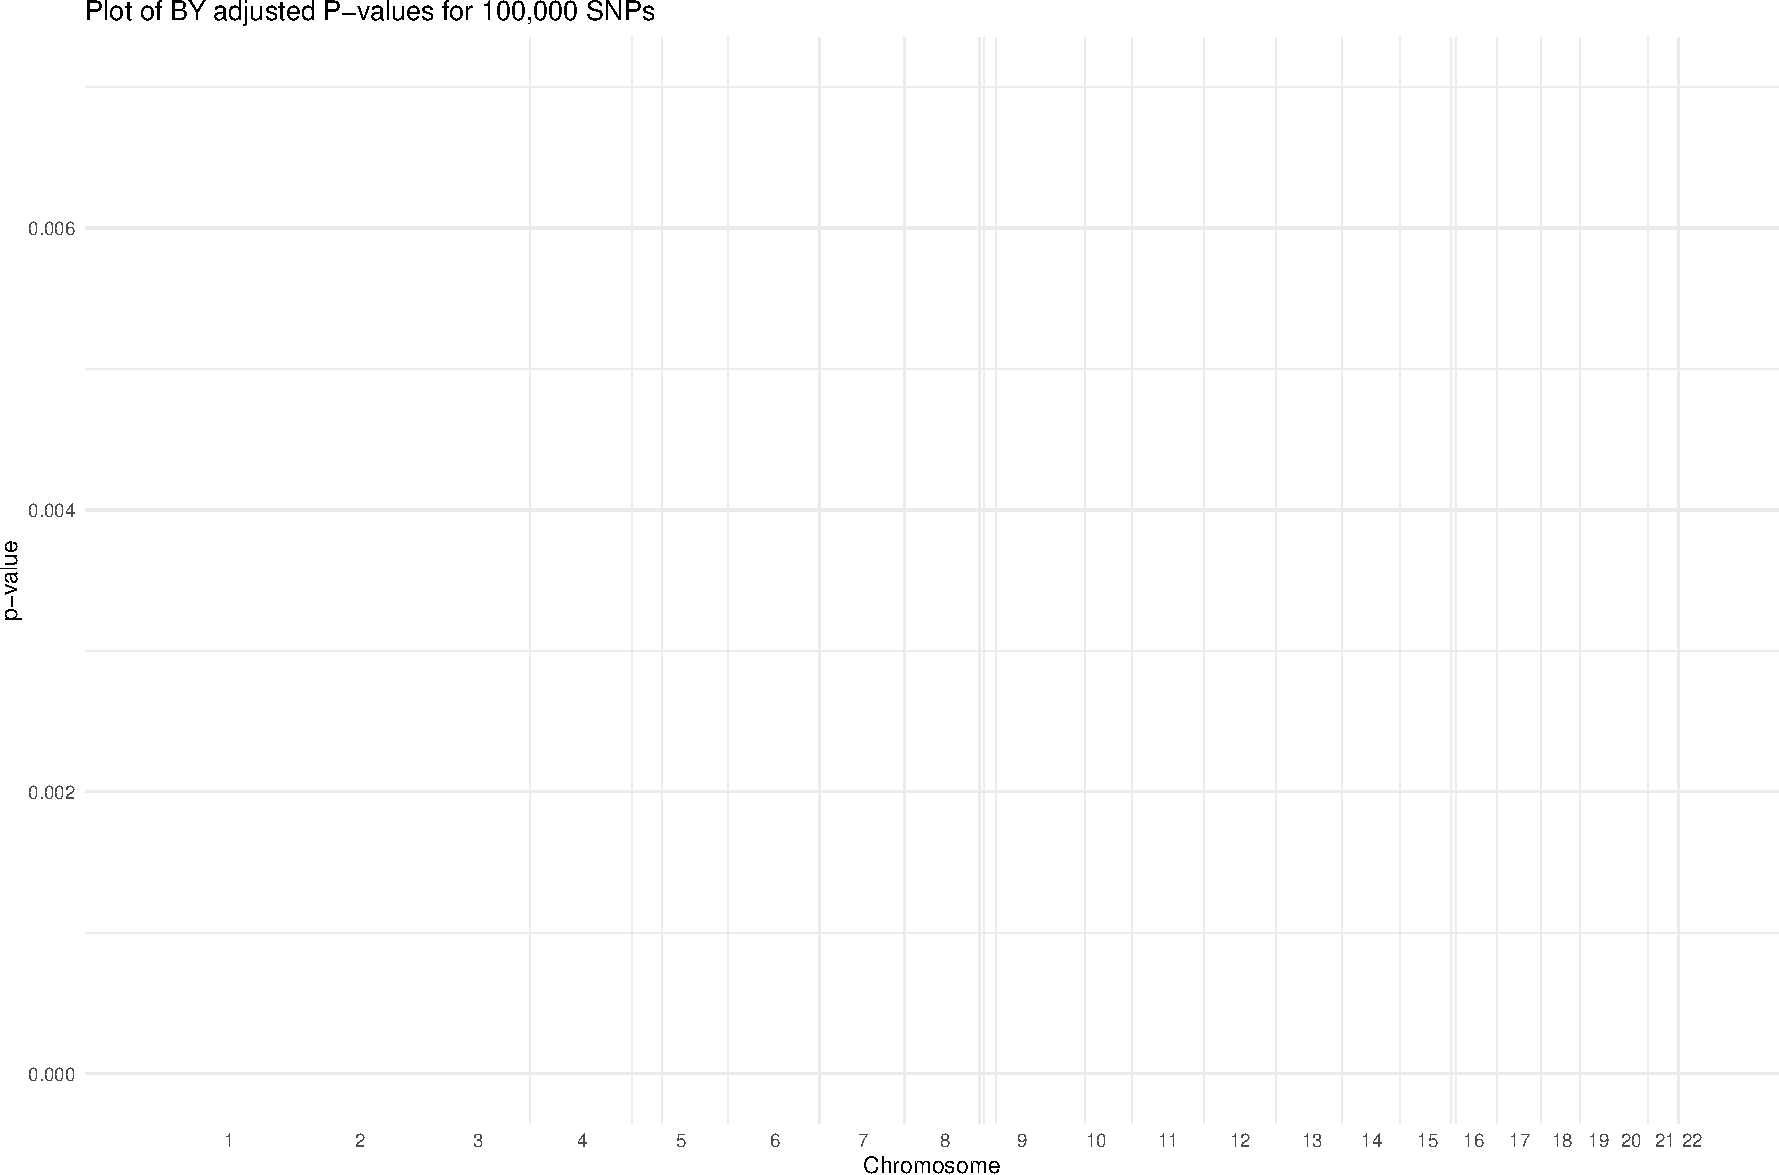
\includegraphics{Arkesh_Das_CMSE_410_Semester_Project_files/figure-latex/BY plot test-1.pdf}

Using my new and improved plotting function, we can see that because the
Benjamini-Yekutieli method is so conservative, all of the p-values were
adjusted to 1.

\subsection{Benjamini-Hochberg}\label{benjamini-hochberg}

Now I will try adjust my p-values using the Benjamini-Hochberg method.

\begin{Shaded}
\begin{Highlighting}[]
\CommentTok{\# Adjusting p\_values using BH}
\NormalTok{df3\_clean}\SpecialCharTok{$}\NormalTok{P\_BH }\OtherTok{\textless{}{-}} \FunctionTok{p.adjust}\NormalTok{(df3\_clean}\SpecialCharTok{$}\NormalTok{P, }\AttributeTok{method =} \StringTok{"BH"}\NormalTok{)}

\CommentTok{\#Summary stats of adjusted p{-}values}
\FunctionTok{summary}\NormalTok{(df3\_clean}\SpecialCharTok{$}\NormalTok{P\_BH)}
\end{Highlighting}
\end{Shaded}

\begin{verbatim}
##    Min. 1st Qu.  Median    Mean 3rd Qu.    Max. 
##  0.9943  0.9943  0.9943  0.9950  0.9958  1.0000
\end{verbatim}

\begin{Shaded}
\begin{Highlighting}[]
\NormalTok{df3\_bh\_sig }\OtherTok{\textless{}{-}}\NormalTok{ df3\_clean }\SpecialCharTok{\%\textgreater{}\%} \FunctionTok{filter}\NormalTok{(P\_BH }\SpecialCharTok{\textless{}} \FloatTok{0.05}\NormalTok{) }\CommentTok{\#there are no significant p{-}values after BH adjustment }
\NormalTok{df3\_clean}\SpecialCharTok{$}\NormalTok{log10\_P\_BH }\OtherTok{\textless{}{-}} \SpecialCharTok{{-}}\FunctionTok{log10}\NormalTok{(df3\_clean}\SpecialCharTok{$}\NormalTok{P\_BH)}

\FunctionTok{manhattan}\NormalTok{(df3\_clean, }\AttributeTok{chr =} \StringTok{"\#CHROM"}\NormalTok{, }\AttributeTok{bp =} \StringTok{"POS"}\NormalTok{, }\AttributeTok{snp =} \StringTok{"ID"}\NormalTok{, }\AttributeTok{p =} \StringTok{"P\_BH"}\NormalTok{, }\AttributeTok{suggestiveline =} \ConstantTok{FALSE}\NormalTok{, }\AttributeTok{ylim =} \FunctionTok{c}\NormalTok{(}\DecValTok{0}\NormalTok{, }\FloatTok{0.005}\NormalTok{)) }
\FunctionTok{title}\NormalTok{(}\AttributeTok{main =} \StringTok{"Plot of BH adjusted P{-}values for 100,000 SNPs"}\NormalTok{)}
\end{Highlighting}
\end{Shaded}

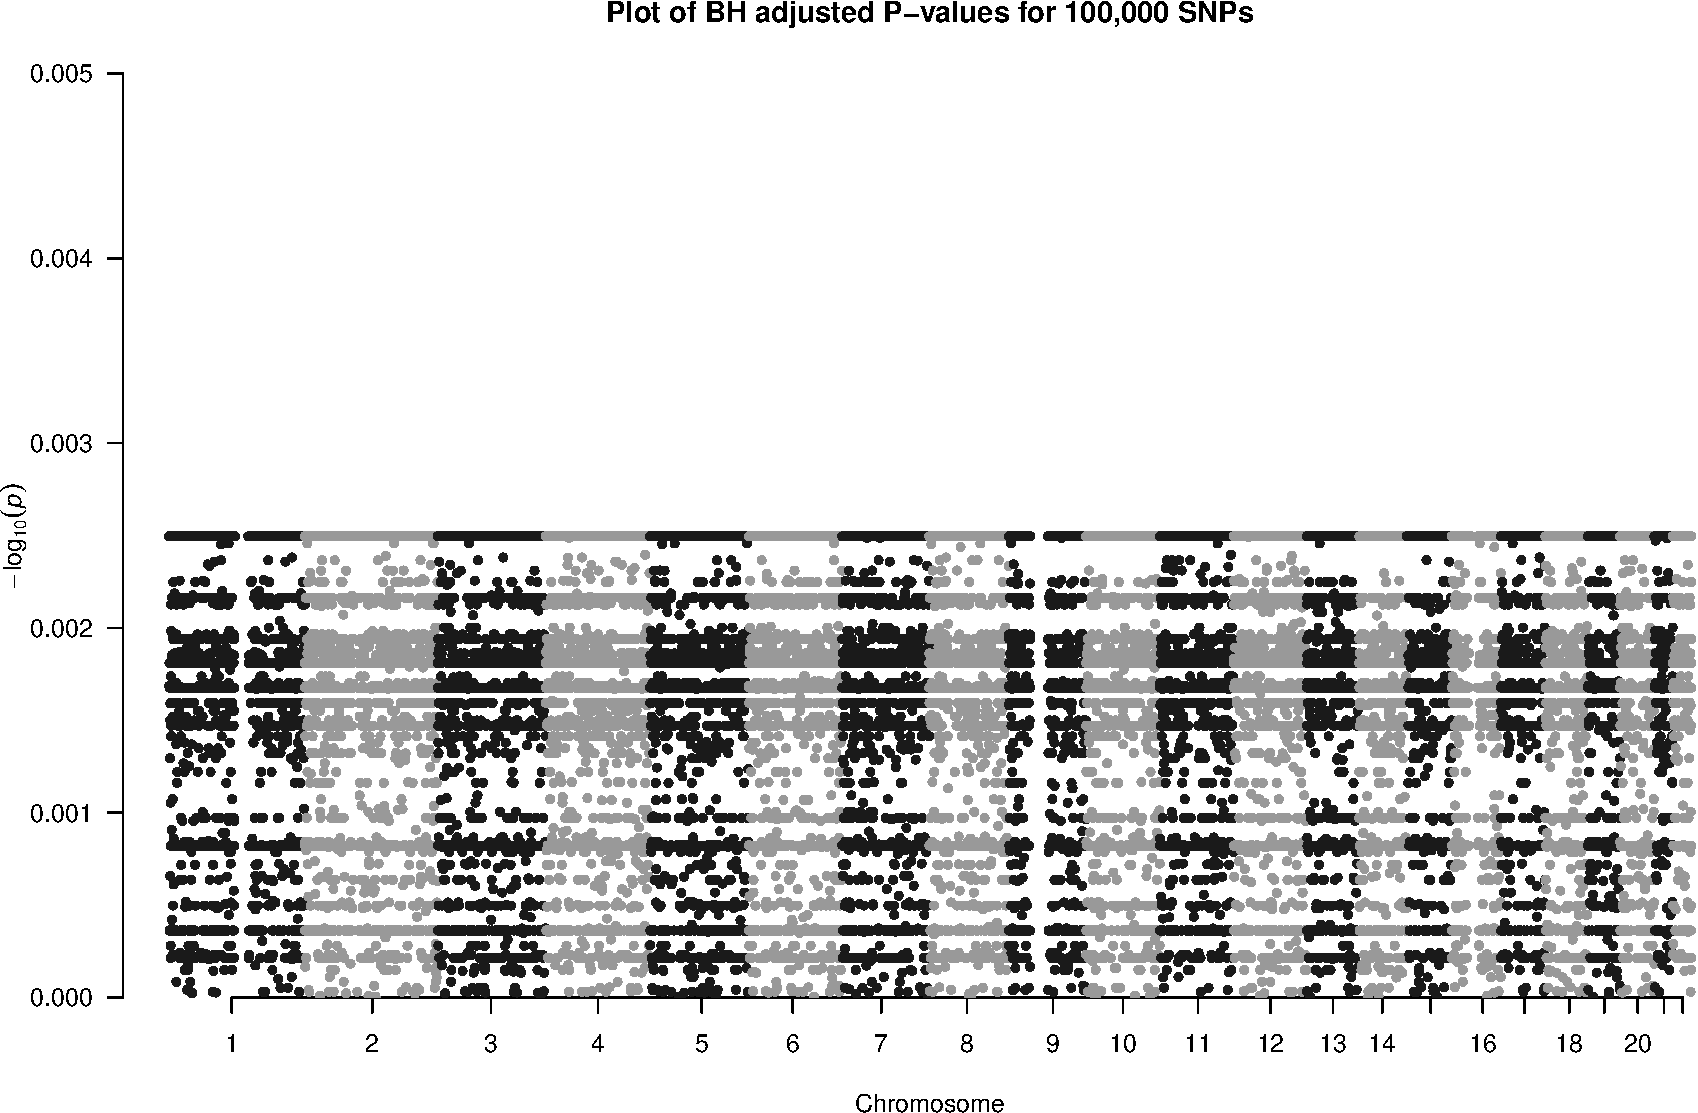
\includegraphics{Arkesh_Das_CMSE_410_Semester_Project_files/figure-latex/Benjamini-Hochberg test-1.pdf}

\begin{Shaded}
\begin{Highlighting}[]
\FunctionTok{generate\_plot}\NormalTok{(df3\_clean, }\AttributeTok{pval\_col =} \StringTok{"P\_BH"}\NormalTok{, }\AttributeTok{plot\_title =} \StringTok{"Plot of BH adjusted P{-}values for 100,000 SNPs"}\NormalTok{)}
\end{Highlighting}
\end{Shaded}

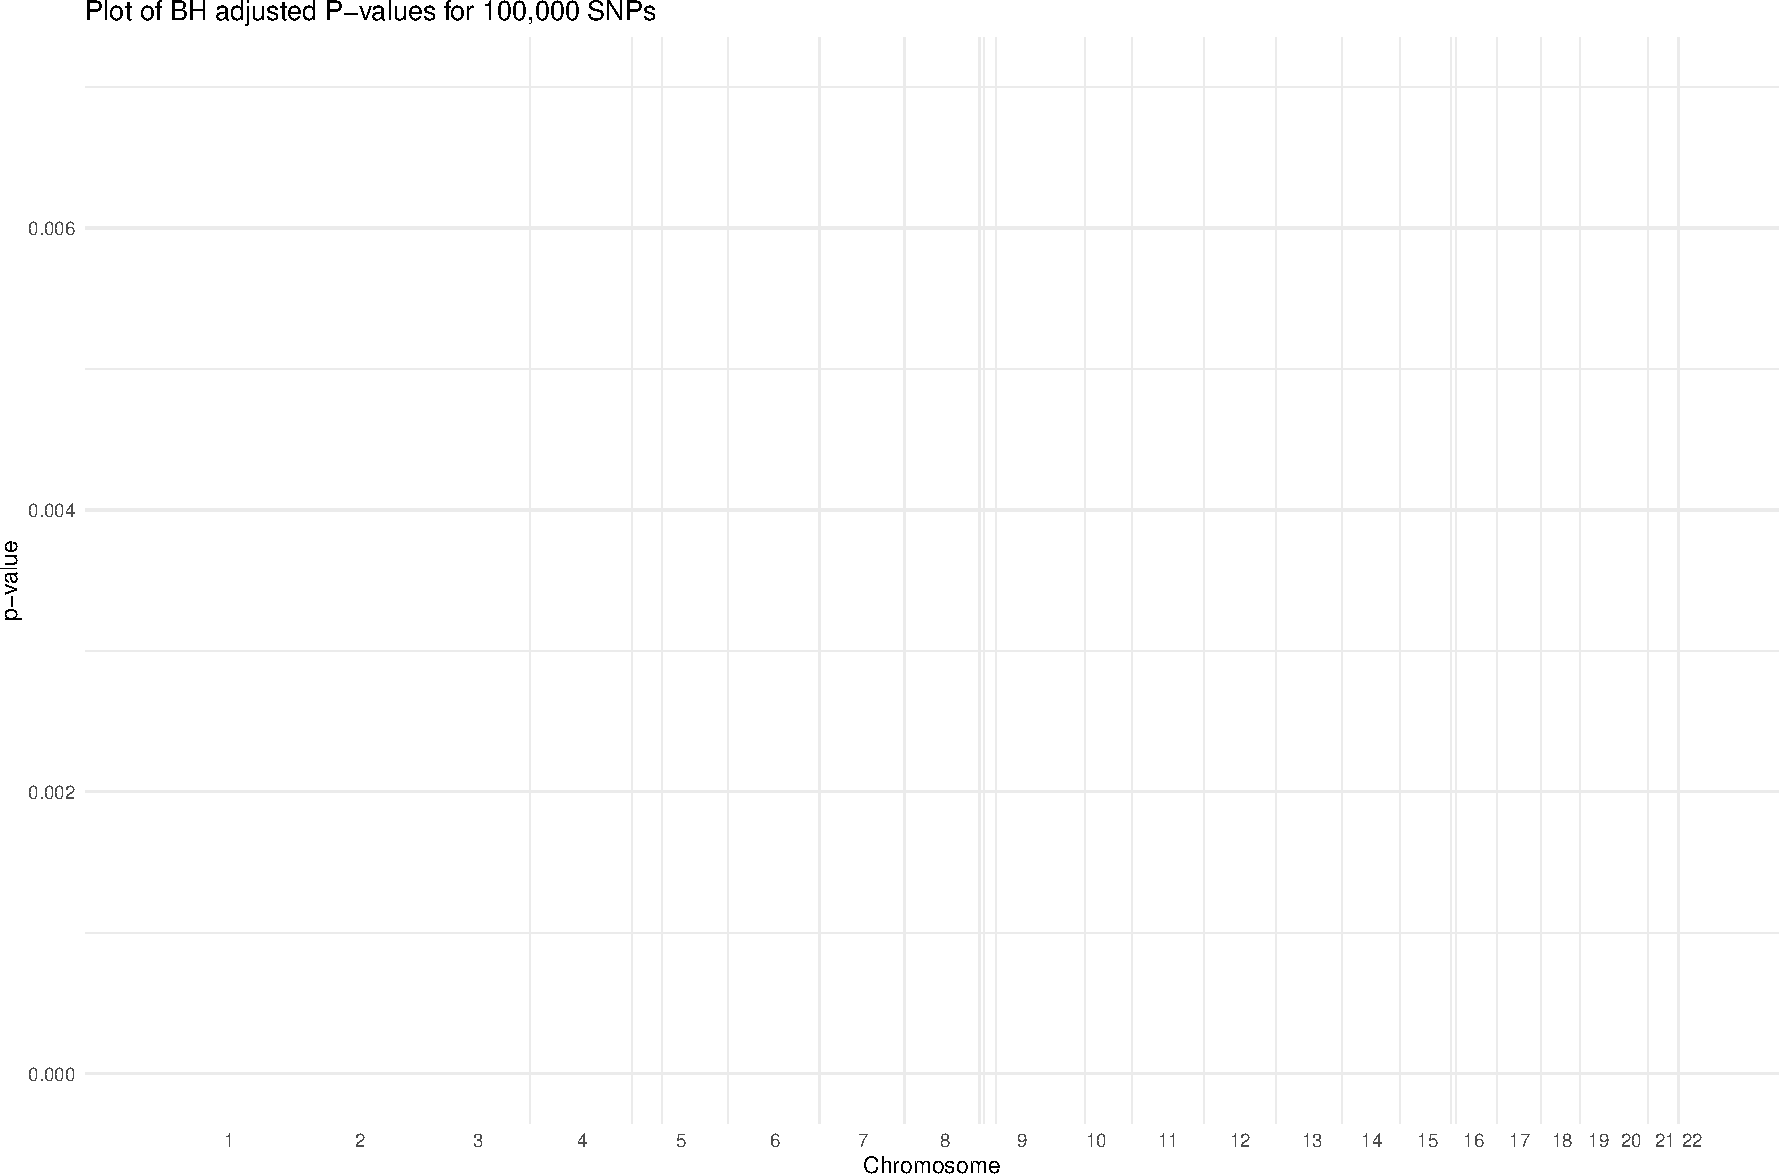
\includegraphics{Arkesh_Das_CMSE_410_Semester_Project_files/figure-latex/BH plot test-1.pdf}

\subsection{Benjamini-Krieger-Yekutieli}\label{benjamini-krieger-yekutieli}

Now I will try to use the Benjamini-Krieger-Yekutieli method in the
\texttt{mutoss} package {[}4{]}:

\begin{Shaded}
\begin{Highlighting}[]
\NormalTok{mutoss}\SpecialCharTok{::}\FunctionTok{loadMethod}\NormalTok{(}\StringTok{"BKY"}\NormalTok{)}


\NormalTok{bky\_result }\OtherTok{\textless{}{-}}\NormalTok{ mutoss}\SpecialCharTok{::}\FunctionTok{runMethod}\NormalTok{(}\StringTok{"BKY"}\NormalTok{, }\FunctionTok{list}\NormalTok{(}\AttributeTok{pValues =}\NormalTok{ df3\_clean}\SpecialCharTok{$}\NormalTok{P, }\AttributeTok{alpha =} \FloatTok{0.05}\NormalTok{))}
\end{Highlighting}
\end{Shaded}

Unfortunately, I could not get the \texttt{mutoss} package's
implementation of BKY to work, so I will instead follow the original
2006 paper {[}5{]}, which describes how to implement the BKY method:

\begin{Shaded}
\begin{Highlighting}[]
\CommentTok{\#BYK function}
\NormalTok{bky\_adjust }\OtherTok{\textless{}{-}} \ControlFlowTok{function}\NormalTok{(p, }\AttributeTok{alpha =} \FloatTok{0.05}\NormalTok{) \{}
\NormalTok{  m }\OtherTok{\textless{}{-}} \FunctionTok{length}\NormalTok{(p)}
\NormalTok{  p\_order }\OtherTok{\textless{}{-}} \FunctionTok{order}\NormalTok{(p)}
\NormalTok{  p\_sorted }\OtherTok{\textless{}{-}}\NormalTok{ p[p\_order]}
\NormalTok{  k }\OtherTok{\textless{}{-}}\NormalTok{ m}\SpecialCharTok{:}\DecValTok{1}
\NormalTok{  c\_m }\OtherTok{\textless{}{-}} \FunctionTok{sum}\NormalTok{(}\DecValTok{1} \SpecialCharTok{/}\NormalTok{ (}\DecValTok{1}\SpecialCharTok{:}\NormalTok{m))}
  
\NormalTok{  thresh }\OtherTok{\textless{}{-}}\NormalTok{ (k }\SpecialCharTok{/}\NormalTok{ m) }\SpecialCharTok{*}\NormalTok{ (alpha }\SpecialCharTok{/}\NormalTok{ (}\DecValTok{1} \SpecialCharTok{+}\NormalTok{ alpha)) }\SpecialCharTok{*}\NormalTok{ (}\DecValTok{1} \SpecialCharTok{/}\NormalTok{ c\_m)}
\NormalTok{  test }\OtherTok{\textless{}{-}}\NormalTok{ p\_sorted }\SpecialCharTok{\textless{}=}\NormalTok{ thresh}
\NormalTok{  max\_k }\OtherTok{\textless{}{-}} \ControlFlowTok{if}\NormalTok{ (}\FunctionTok{any}\NormalTok{(test)) }\FunctionTok{max}\NormalTok{(}\FunctionTok{which}\NormalTok{(test)) }\ControlFlowTok{else} \DecValTok{0}
  
\NormalTok{  adjusted }\OtherTok{\textless{}{-}} \FunctionTok{rep}\NormalTok{(}\DecValTok{1}\NormalTok{, m)}
  \ControlFlowTok{if}\NormalTok{ (max\_k }\SpecialCharTok{\textgreater{}} \DecValTok{0}\NormalTok{) \{}
\NormalTok{    adjusted[p\_order[}\DecValTok{1}\SpecialCharTok{:}\NormalTok{max\_k]] }\OtherTok{\textless{}{-}} \FunctionTok{pmin}\NormalTok{(}\DecValTok{1}\NormalTok{, thresh[max\_k])}
\NormalTok{  \}}
  
  \FunctionTok{return}\NormalTok{(adjusted)}
\NormalTok{\}}

\CommentTok{\# Applying BKY to the data}

\NormalTok{df3\_clean}\SpecialCharTok{$}\NormalTok{P\_BKY }\OtherTok{\textless{}{-}} \FunctionTok{bky\_adjust}\NormalTok{(df3\_clean}\SpecialCharTok{$}\NormalTok{P, }\AttributeTok{alpha =} \FloatTok{0.05}\NormalTok{)}
\NormalTok{df3\_bky\_sig }\OtherTok{\textless{}{-}}\NormalTok{ df3\_clean }\SpecialCharTok{\%\textgreater{}\%} \FunctionTok{filter}\NormalTok{(P\_BKY }\SpecialCharTok{\textless{}} \FloatTok{0.05}\NormalTok{)}

\FunctionTok{summary}\NormalTok{(df3\_bky\_sig}\SpecialCharTok{$}\NormalTok{P\_BKY)}
\end{Highlighting}
\end{Shaded}

\begin{verbatim}
##     Min.  1st Qu.   Median     Mean  3rd Qu.     Max. 
## 0.003935 0.003935 0.003935 0.003935 0.003935 0.003935
\end{verbatim}

\begin{Shaded}
\begin{Highlighting}[]
\CommentTok{\# Plot}
\FunctionTok{manhattan}\NormalTok{(df3\_clean, }\AttributeTok{chr =} \StringTok{"\#CHROM"}\NormalTok{, }\AttributeTok{bp =} \StringTok{"POS"}\NormalTok{, }\AttributeTok{snp =} \StringTok{"ID"}\NormalTok{, }\AttributeTok{p =} \StringTok{"P\_BKY"}\NormalTok{,}
          \AttributeTok{suggestiveline =} \ConstantTok{FALSE}\NormalTok{)}
\FunctionTok{title}\NormalTok{(}\AttributeTok{main =} \StringTok{"Plot of BKY Adjusted P{-}values for 100,000 SNPs"}\NormalTok{)}
\end{Highlighting}
\end{Shaded}

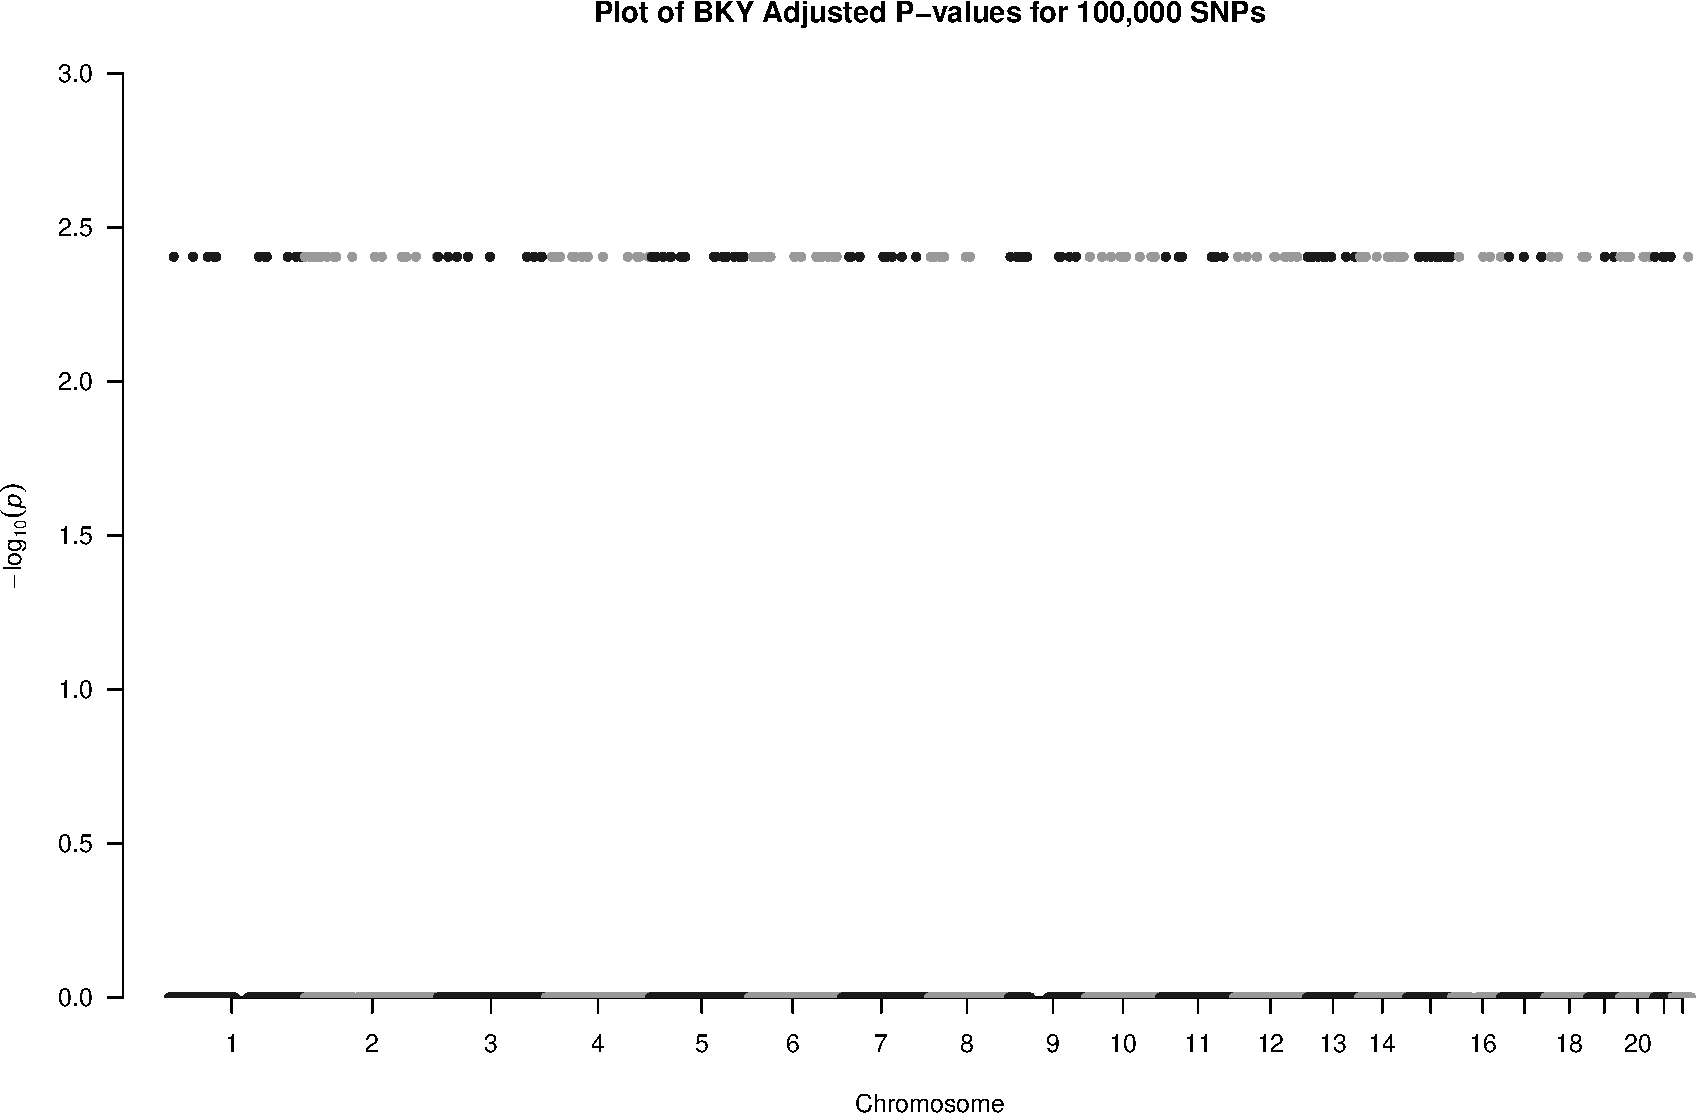
\includegraphics{Arkesh_Das_CMSE_410_Semester_Project_files/figure-latex/BKY implementation-1.pdf}

\begin{Shaded}
\begin{Highlighting}[]
\FunctionTok{generate\_plot}\NormalTok{(df3\_clean, }\AttributeTok{pval\_col =} \StringTok{"P\_BKY"}\NormalTok{, }\AttributeTok{plot\_title =} \StringTok{"Plot of BKY adjusted P{-}values for 100,000 SNPs"}\NormalTok{)}
\end{Highlighting}
\end{Shaded}

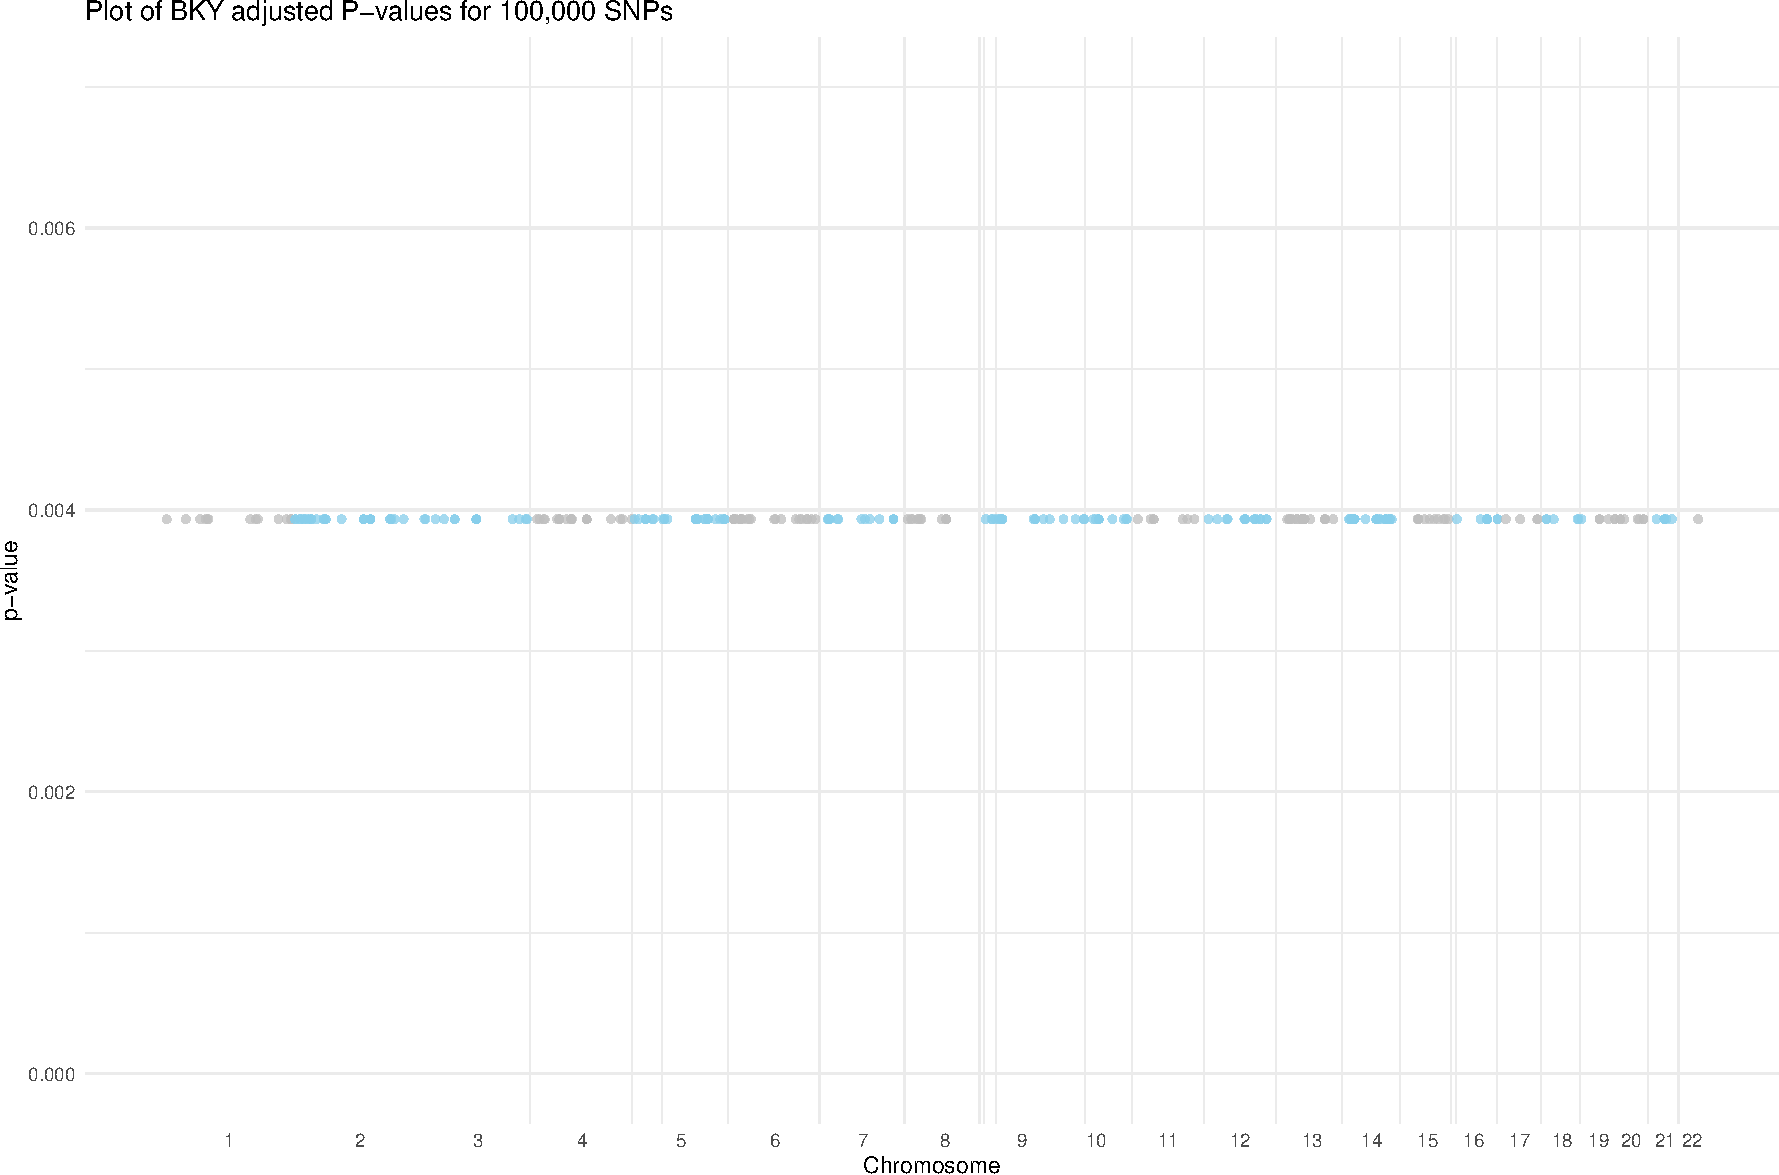
\includegraphics{Arkesh_Das_CMSE_410_Semester_Project_files/figure-latex/BYK plot test-1.pdf}
This time, I was able to isolate around 300 significant SNPs using the
BYK method. However, they were all the same p-value. Therefore, while
BYK is able to separate\\
\#\# Storey-Tibshirani (q-value)

Now I will be adjusting my p-values using the Storey-Tibshirani method
{[}6{]}. Thankfully, there is a package in R that was designed in
collaboration with the creators of this method, the \texttt{qvalue}
package. I followed the documentation of the \texttt{qvalue} package to
use the \texttt{qvalue()} method and other methods on my data {[}7{]}.

\begin{Shaded}
\begin{Highlighting}[]
\NormalTok{qobj }\OtherTok{\textless{}{-}} \FunctionTok{qvalue}\NormalTok{(}\AttributeTok{p =}\NormalTok{ df3\_clean}\SpecialCharTok{$}\NormalTok{P)  }\CommentTok{\# estimating pi\_0 and q{-}values}
\NormalTok{df3\_clean}\SpecialCharTok{$}\NormalTok{q\_value }\OtherTok{\textless{}{-}}\NormalTok{ qobj}\SpecialCharTok{$}\NormalTok{qvalues}

\NormalTok{df3\_q\_sig }\OtherTok{\textless{}{-}}\NormalTok{ df3\_clean }\SpecialCharTok{\%\textgreater{}\%} \FunctionTok{filter}\NormalTok{(q\_value }\SpecialCharTok{\textless{}} \FloatTok{0.05}\NormalTok{)}
\FunctionTok{nrow}\NormalTok{(df3\_q\_sig)  }
\end{Highlighting}
\end{Shaded}

\begin{verbatim}
## [1] 0
\end{verbatim}

\begin{Shaded}
\begin{Highlighting}[]
\NormalTok{qobj}\SpecialCharTok{$}\NormalTok{pi0}
\end{Highlighting}
\end{Shaded}

\begin{verbatim}
## [1] 0.9716845
\end{verbatim}

Unfortunately, I was not able to actually find any significant
q\_values. My pi\_0 was 0.971, which means that 97.1\% of the tested
SNPs are estimated to be null.

\begin{Shaded}
\begin{Highlighting}[]
\NormalTok{top\_bky }\OtherTok{\textless{}{-}}\NormalTok{ df3\_clean }\SpecialCharTok{\%\textgreater{}\%}
  \FunctionTok{arrange}\NormalTok{(P) }\SpecialCharTok{\%\textgreater{}\%}
  \FunctionTok{slice}\NormalTok{(}\DecValTok{1}\SpecialCharTok{:}\DecValTok{50}\NormalTok{) }\SpecialCharTok{\%\textgreater{}\%}
  \FunctionTok{select}\NormalTok{(}\StringTok{\textasciigrave{}}\AttributeTok{\#CHROM}\StringTok{\textasciigrave{}}\NormalTok{, POS, ID, P, P\_BKY)}
\end{Highlighting}
\end{Shaded}

Taking a second look at the p-values that were marked as being
signficant from BYK, they appear to be randomly clustered throughout the
genome. However, the second most significant SNP is located on
chromosome 6, the same chromosome as the HLA gene cluster that was found
to be significant in the original study. So, I think to conclude, I will
try to figure out where this SNP is located and its potential biological
function.

SNP POS: 129948488 \#CHROM: 6

I used the NCBI Human Genome Data Viewer {[}8{]} to figure out the
genomic context of chr6:129948488. This SNP lies within an intron region
of L3MBTL3, situated between a nearby HLA class II gene and an
uncharacterized gene. L3MBTL3 has been implicated in several GWAS as
influencing hematopoietic traits and immunoglobulin A (IgA) levels.
Variants in L3MBTL3 have been associated with natural variation in IgA
concentrations, suggesting a potential role in humoral immune
regulation. These findings suggest that SNPs in or near L3MBTL3 could
indirectly modulate immune responses, potentially by influencing the
development or regulation of immune effector cells {[}9{]}.

Therefore, while I was not able to identify a clear enrichment of
significant SNPs in known immune loci across the genome, I was able to
pinpoint at least one biologically plausible candidate. Its proximity to
the HLA region and its known association with immune-related traits make
it a promising lead for further investigation. Further analysis of the
SNPs that were flagged as being significant by the BKY method should be
looked into, as they may represent novel loci of biological relevance
that have not yet been characterized in the context of immune response
by the original study.

\#Misc graphs

\begin{Shaded}
\begin{Highlighting}[]
\NormalTok{df3\_clean}\SpecialCharTok{$}\NormalTok{logP }\OtherTok{\textless{}{-}} \SpecialCharTok{{-}}\FunctionTok{log10}\NormalTok{(df3\_clean}\SpecialCharTok{$}\NormalTok{P)}


\FunctionTok{ggplot}\NormalTok{(df3\_clean, }\FunctionTok{aes}\NormalTok{(}\AttributeTok{x =} \SpecialCharTok{{-}}\FunctionTok{log10}\NormalTok{(P))) }\SpecialCharTok{+}
  \FunctionTok{geom\_histogram}\NormalTok{(}\AttributeTok{bins =} \DecValTok{50}\NormalTok{, }\AttributeTok{fill =} \StringTok{"skyblue"}\NormalTok{, }\AttributeTok{color =} \StringTok{"white"}\NormalTok{) }\SpecialCharTok{+}
  \FunctionTok{labs}\NormalTok{(}\AttributeTok{title =} \StringTok{"Distribution of –log10(P{-}values)"}\NormalTok{,}
       \AttributeTok{x =} \StringTok{"–log10(P{-}value)"}\NormalTok{, }\AttributeTok{y =} \StringTok{"Count"}\NormalTok{) }\SpecialCharTok{+}\FunctionTok{xlim}\NormalTok{(}\DecValTok{0}\NormalTok{, }\DecValTok{4}\NormalTok{) }
\end{Highlighting}
\end{Shaded}

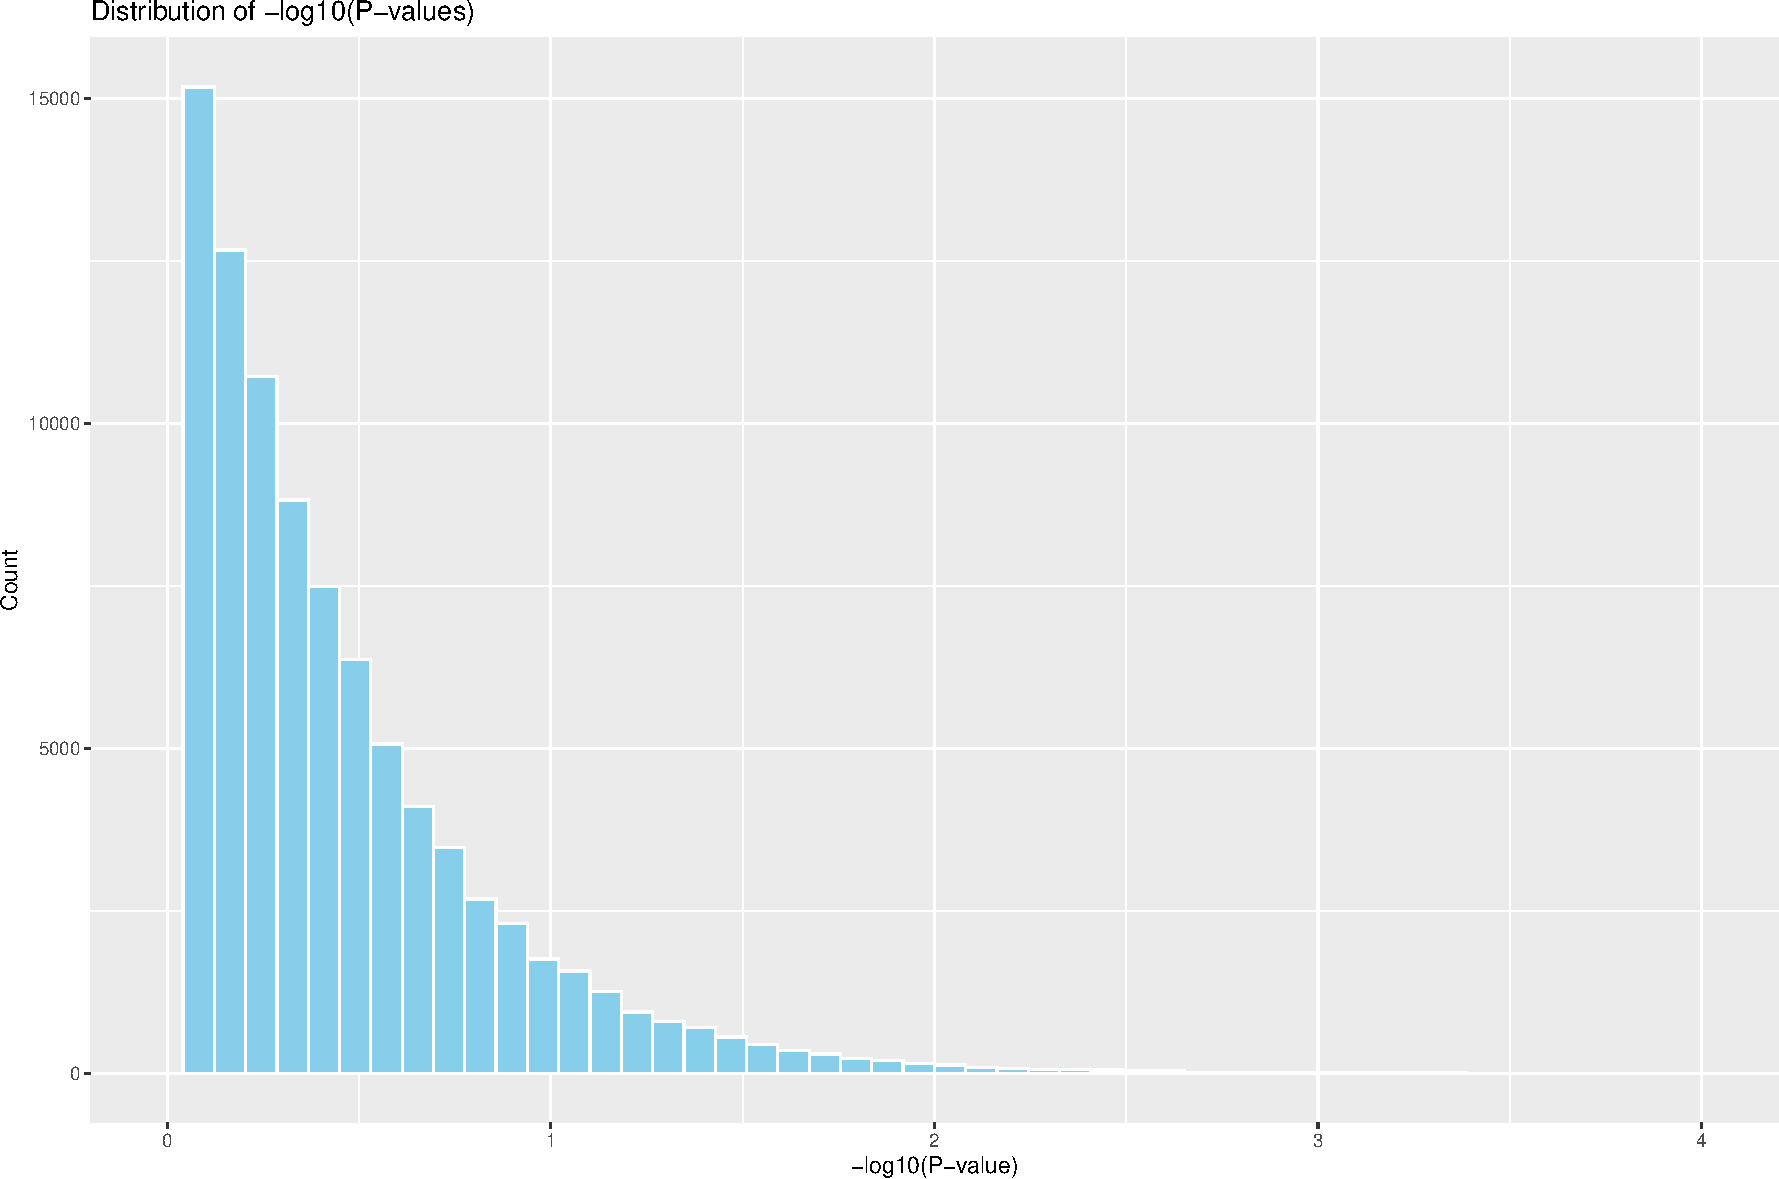
\includegraphics{Arkesh_Das_CMSE_410_Semester_Project_files/figure-latex/normal distribution testing-1.pdf}

\begin{Shaded}
\begin{Highlighting}[]
  \FunctionTok{theme\_minimal}\NormalTok{()}
\end{Highlighting}
\end{Shaded}

\begin{verbatim}
## List of 136
##  $ line                            :List of 6
##   ..$ colour       : chr "black"
##   ..$ linewidth    : num 0.5
##   ..$ linetype     : num 1
##   ..$ lineend      : chr "butt"
##   ..$ arrow        : logi FALSE
##   ..$ inherit.blank: logi TRUE
##   ..- attr(*, "class")= chr [1:2] "element_line" "element"
##  $ rect                            :List of 5
##   ..$ fill         : chr "white"
##   ..$ colour       : chr "black"
##   ..$ linewidth    : num 0.5
##   ..$ linetype     : num 1
##   ..$ inherit.blank: logi TRUE
##   ..- attr(*, "class")= chr [1:2] "element_rect" "element"
##  $ text                            :List of 11
##   ..$ family       : chr ""
##   ..$ face         : chr "plain"
##   ..$ colour       : chr "black"
##   ..$ size         : num 11
##   ..$ hjust        : num 0.5
##   ..$ vjust        : num 0.5
##   ..$ angle        : num 0
##   ..$ lineheight   : num 0.9
##   ..$ margin       : 'margin' num [1:4] 0points 0points 0points 0points
##   .. ..- attr(*, "unit")= int 8
##   ..$ debug        : logi FALSE
##   ..$ inherit.blank: logi TRUE
##   ..- attr(*, "class")= chr [1:2] "element_text" "element"
##  $ title                           : NULL
##  $ aspect.ratio                    : NULL
##  $ axis.title                      : NULL
##  $ axis.title.x                    :List of 11
##   ..$ family       : NULL
##   ..$ face         : NULL
##   ..$ colour       : NULL
##   ..$ size         : NULL
##   ..$ hjust        : NULL
##   ..$ vjust        : num 1
##   ..$ angle        : NULL
##   ..$ lineheight   : NULL
##   ..$ margin       : 'margin' num [1:4] 2.75points 0points 0points 0points
##   .. ..- attr(*, "unit")= int 8
##   ..$ debug        : NULL
##   ..$ inherit.blank: logi TRUE
##   ..- attr(*, "class")= chr [1:2] "element_text" "element"
##  $ axis.title.x.top                :List of 11
##   ..$ family       : NULL
##   ..$ face         : NULL
##   ..$ colour       : NULL
##   ..$ size         : NULL
##   ..$ hjust        : NULL
##   ..$ vjust        : num 0
##   ..$ angle        : NULL
##   ..$ lineheight   : NULL
##   ..$ margin       : 'margin' num [1:4] 0points 0points 2.75points 0points
##   .. ..- attr(*, "unit")= int 8
##   ..$ debug        : NULL
##   ..$ inherit.blank: logi TRUE
##   ..- attr(*, "class")= chr [1:2] "element_text" "element"
##  $ axis.title.x.bottom             : NULL
##  $ axis.title.y                    :List of 11
##   ..$ family       : NULL
##   ..$ face         : NULL
##   ..$ colour       : NULL
##   ..$ size         : NULL
##   ..$ hjust        : NULL
##   ..$ vjust        : num 1
##   ..$ angle        : num 90
##   ..$ lineheight   : NULL
##   ..$ margin       : 'margin' num [1:4] 0points 2.75points 0points 0points
##   .. ..- attr(*, "unit")= int 8
##   ..$ debug        : NULL
##   ..$ inherit.blank: logi TRUE
##   ..- attr(*, "class")= chr [1:2] "element_text" "element"
##  $ axis.title.y.left               : NULL
##  $ axis.title.y.right              :List of 11
##   ..$ family       : NULL
##   ..$ face         : NULL
##   ..$ colour       : NULL
##   ..$ size         : NULL
##   ..$ hjust        : NULL
##   ..$ vjust        : num 1
##   ..$ angle        : num -90
##   ..$ lineheight   : NULL
##   ..$ margin       : 'margin' num [1:4] 0points 0points 0points 2.75points
##   .. ..- attr(*, "unit")= int 8
##   ..$ debug        : NULL
##   ..$ inherit.blank: logi TRUE
##   ..- attr(*, "class")= chr [1:2] "element_text" "element"
##  $ axis.text                       :List of 11
##   ..$ family       : NULL
##   ..$ face         : NULL
##   ..$ colour       : chr "grey30"
##   ..$ size         : 'rel' num 0.8
##   ..$ hjust        : NULL
##   ..$ vjust        : NULL
##   ..$ angle        : NULL
##   ..$ lineheight   : NULL
##   ..$ margin       : NULL
##   ..$ debug        : NULL
##   ..$ inherit.blank: logi TRUE
##   ..- attr(*, "class")= chr [1:2] "element_text" "element"
##  $ axis.text.x                     :List of 11
##   ..$ family       : NULL
##   ..$ face         : NULL
##   ..$ colour       : NULL
##   ..$ size         : NULL
##   ..$ hjust        : NULL
##   ..$ vjust        : num 1
##   ..$ angle        : NULL
##   ..$ lineheight   : NULL
##   ..$ margin       : 'margin' num [1:4] 2.2points 0points 0points 0points
##   .. ..- attr(*, "unit")= int 8
##   ..$ debug        : NULL
##   ..$ inherit.blank: logi TRUE
##   ..- attr(*, "class")= chr [1:2] "element_text" "element"
##  $ axis.text.x.top                 :List of 11
##   ..$ family       : NULL
##   ..$ face         : NULL
##   ..$ colour       : NULL
##   ..$ size         : NULL
##   ..$ hjust        : NULL
##   ..$ vjust        : num 0
##   ..$ angle        : NULL
##   ..$ lineheight   : NULL
##   ..$ margin       : 'margin' num [1:4] 0points 0points 2.2points 0points
##   .. ..- attr(*, "unit")= int 8
##   ..$ debug        : NULL
##   ..$ inherit.blank: logi TRUE
##   ..- attr(*, "class")= chr [1:2] "element_text" "element"
##  $ axis.text.x.bottom              : NULL
##  $ axis.text.y                     :List of 11
##   ..$ family       : NULL
##   ..$ face         : NULL
##   ..$ colour       : NULL
##   ..$ size         : NULL
##   ..$ hjust        : num 1
##   ..$ vjust        : NULL
##   ..$ angle        : NULL
##   ..$ lineheight   : NULL
##   ..$ margin       : 'margin' num [1:4] 0points 2.2points 0points 0points
##   .. ..- attr(*, "unit")= int 8
##   ..$ debug        : NULL
##   ..$ inherit.blank: logi TRUE
##   ..- attr(*, "class")= chr [1:2] "element_text" "element"
##  $ axis.text.y.left                : NULL
##  $ axis.text.y.right               :List of 11
##   ..$ family       : NULL
##   ..$ face         : NULL
##   ..$ colour       : NULL
##   ..$ size         : NULL
##   ..$ hjust        : num 0
##   ..$ vjust        : NULL
##   ..$ angle        : NULL
##   ..$ lineheight   : NULL
##   ..$ margin       : 'margin' num [1:4] 0points 0points 0points 2.2points
##   .. ..- attr(*, "unit")= int 8
##   ..$ debug        : NULL
##   ..$ inherit.blank: logi TRUE
##   ..- attr(*, "class")= chr [1:2] "element_text" "element"
##  $ axis.text.theta                 : NULL
##  $ axis.text.r                     :List of 11
##   ..$ family       : NULL
##   ..$ face         : NULL
##   ..$ colour       : NULL
##   ..$ size         : NULL
##   ..$ hjust        : num 0.5
##   ..$ vjust        : NULL
##   ..$ angle        : NULL
##   ..$ lineheight   : NULL
##   ..$ margin       : 'margin' num [1:4] 0points 2.2points 0points 2.2points
##   .. ..- attr(*, "unit")= int 8
##   ..$ debug        : NULL
##   ..$ inherit.blank: logi TRUE
##   ..- attr(*, "class")= chr [1:2] "element_text" "element"
##  $ axis.ticks                      : list()
##   ..- attr(*, "class")= chr [1:2] "element_blank" "element"
##  $ axis.ticks.x                    : NULL
##  $ axis.ticks.x.top                : NULL
##  $ axis.ticks.x.bottom             : NULL
##  $ axis.ticks.y                    : NULL
##  $ axis.ticks.y.left               : NULL
##  $ axis.ticks.y.right              : NULL
##  $ axis.ticks.theta                : NULL
##  $ axis.ticks.r                    : NULL
##  $ axis.minor.ticks.x.top          : NULL
##  $ axis.minor.ticks.x.bottom       : NULL
##  $ axis.minor.ticks.y.left         : NULL
##  $ axis.minor.ticks.y.right        : NULL
##  $ axis.minor.ticks.theta          : NULL
##  $ axis.minor.ticks.r              : NULL
##  $ axis.ticks.length               : 'simpleUnit' num 2.75points
##   ..- attr(*, "unit")= int 8
##  $ axis.ticks.length.x             : NULL
##  $ axis.ticks.length.x.top         : NULL
##  $ axis.ticks.length.x.bottom      : NULL
##  $ axis.ticks.length.y             : NULL
##  $ axis.ticks.length.y.left        : NULL
##  $ axis.ticks.length.y.right       : NULL
##  $ axis.ticks.length.theta         : NULL
##  $ axis.ticks.length.r             : NULL
##  $ axis.minor.ticks.length         : 'rel' num 0.75
##  $ axis.minor.ticks.length.x       : NULL
##  $ axis.minor.ticks.length.x.top   : NULL
##  $ axis.minor.ticks.length.x.bottom: NULL
##  $ axis.minor.ticks.length.y       : NULL
##  $ axis.minor.ticks.length.y.left  : NULL
##  $ axis.minor.ticks.length.y.right : NULL
##  $ axis.minor.ticks.length.theta   : NULL
##  $ axis.minor.ticks.length.r       : NULL
##  $ axis.line                       : list()
##   ..- attr(*, "class")= chr [1:2] "element_blank" "element"
##  $ axis.line.x                     : NULL
##  $ axis.line.x.top                 : NULL
##  $ axis.line.x.bottom              : NULL
##  $ axis.line.y                     : NULL
##  $ axis.line.y.left                : NULL
##  $ axis.line.y.right               : NULL
##  $ axis.line.theta                 : NULL
##  $ axis.line.r                     : NULL
##  $ legend.background               : list()
##   ..- attr(*, "class")= chr [1:2] "element_blank" "element"
##  $ legend.margin                   : 'margin' num [1:4] 5.5points 5.5points 5.5points 5.5points
##   ..- attr(*, "unit")= int 8
##  $ legend.spacing                  : 'simpleUnit' num 11points
##   ..- attr(*, "unit")= int 8
##  $ legend.spacing.x                : NULL
##  $ legend.spacing.y                : NULL
##  $ legend.key                      : list()
##   ..- attr(*, "class")= chr [1:2] "element_blank" "element"
##  $ legend.key.size                 : 'simpleUnit' num 1.2lines
##   ..- attr(*, "unit")= int 3
##  $ legend.key.height               : NULL
##  $ legend.key.width                : NULL
##  $ legend.key.spacing              : 'simpleUnit' num 5.5points
##   ..- attr(*, "unit")= int 8
##  $ legend.key.spacing.x            : NULL
##  $ legend.key.spacing.y            : NULL
##  $ legend.frame                    : NULL
##  $ legend.ticks                    : NULL
##  $ legend.ticks.length             : 'rel' num 0.2
##  $ legend.axis.line                : NULL
##  $ legend.text                     :List of 11
##   ..$ family       : NULL
##   ..$ face         : NULL
##   ..$ colour       : NULL
##   ..$ size         : 'rel' num 0.8
##   ..$ hjust        : NULL
##   ..$ vjust        : NULL
##   ..$ angle        : NULL
##   ..$ lineheight   : NULL
##   ..$ margin       : NULL
##   ..$ debug        : NULL
##   ..$ inherit.blank: logi TRUE
##   ..- attr(*, "class")= chr [1:2] "element_text" "element"
##  $ legend.text.position            : NULL
##  $ legend.title                    :List of 11
##   ..$ family       : NULL
##   ..$ face         : NULL
##   ..$ colour       : NULL
##   ..$ size         : NULL
##   ..$ hjust        : num 0
##   ..$ vjust        : NULL
##   ..$ angle        : NULL
##   ..$ lineheight   : NULL
##   ..$ margin       : NULL
##   ..$ debug        : NULL
##   ..$ inherit.blank: logi TRUE
##   ..- attr(*, "class")= chr [1:2] "element_text" "element"
##  $ legend.title.position           : NULL
##  $ legend.position                 : chr "right"
##  $ legend.position.inside          : NULL
##  $ legend.direction                : NULL
##  $ legend.byrow                    : NULL
##  $ legend.justification            : chr "center"
##  $ legend.justification.top        : NULL
##  $ legend.justification.bottom     : NULL
##  $ legend.justification.left       : NULL
##  $ legend.justification.right      : NULL
##  $ legend.justification.inside     : NULL
##  $ legend.location                 : NULL
##  $ legend.box                      : NULL
##  $ legend.box.just                 : NULL
##  $ legend.box.margin               : 'margin' num [1:4] 0cm 0cm 0cm 0cm
##   ..- attr(*, "unit")= int 1
##  $ legend.box.background           : list()
##   ..- attr(*, "class")= chr [1:2] "element_blank" "element"
##  $ legend.box.spacing              : 'simpleUnit' num 11points
##   ..- attr(*, "unit")= int 8
##   [list output truncated]
##  - attr(*, "class")= chr [1:2] "theme" "gg"
##  - attr(*, "complete")= logi TRUE
##  - attr(*, "validate")= logi TRUE
\end{verbatim}

\begin{Shaded}
\begin{Highlighting}[]
\FunctionTok{ggplot}\NormalTok{(df3\_clean, }\FunctionTok{aes}\NormalTok{(}\AttributeTok{x =} \SpecialCharTok{{-}}\FunctionTok{log10}\NormalTok{(P))) }\SpecialCharTok{+}
  \FunctionTok{geom\_histogram}\NormalTok{(}\AttributeTok{bins =} \DecValTok{50}\NormalTok{, }\AttributeTok{fill =} \StringTok{"skyblue"}\NormalTok{, }\AttributeTok{color =} \StringTok{"white"}\NormalTok{) }\SpecialCharTok{+}
  \FunctionTok{labs}\NormalTok{(}\AttributeTok{title =} \StringTok{"Distribution of –log10(P{-}values)"}\NormalTok{,}
       \AttributeTok{x =} \StringTok{"–log10(P{-}value)"}\NormalTok{, }\AttributeTok{y =} \StringTok{"Count"}\NormalTok{) }\SpecialCharTok{+}\FunctionTok{xlim}\NormalTok{(}\DecValTok{2}\NormalTok{, }\DecValTok{4}\NormalTok{) }
\end{Highlighting}
\end{Shaded}

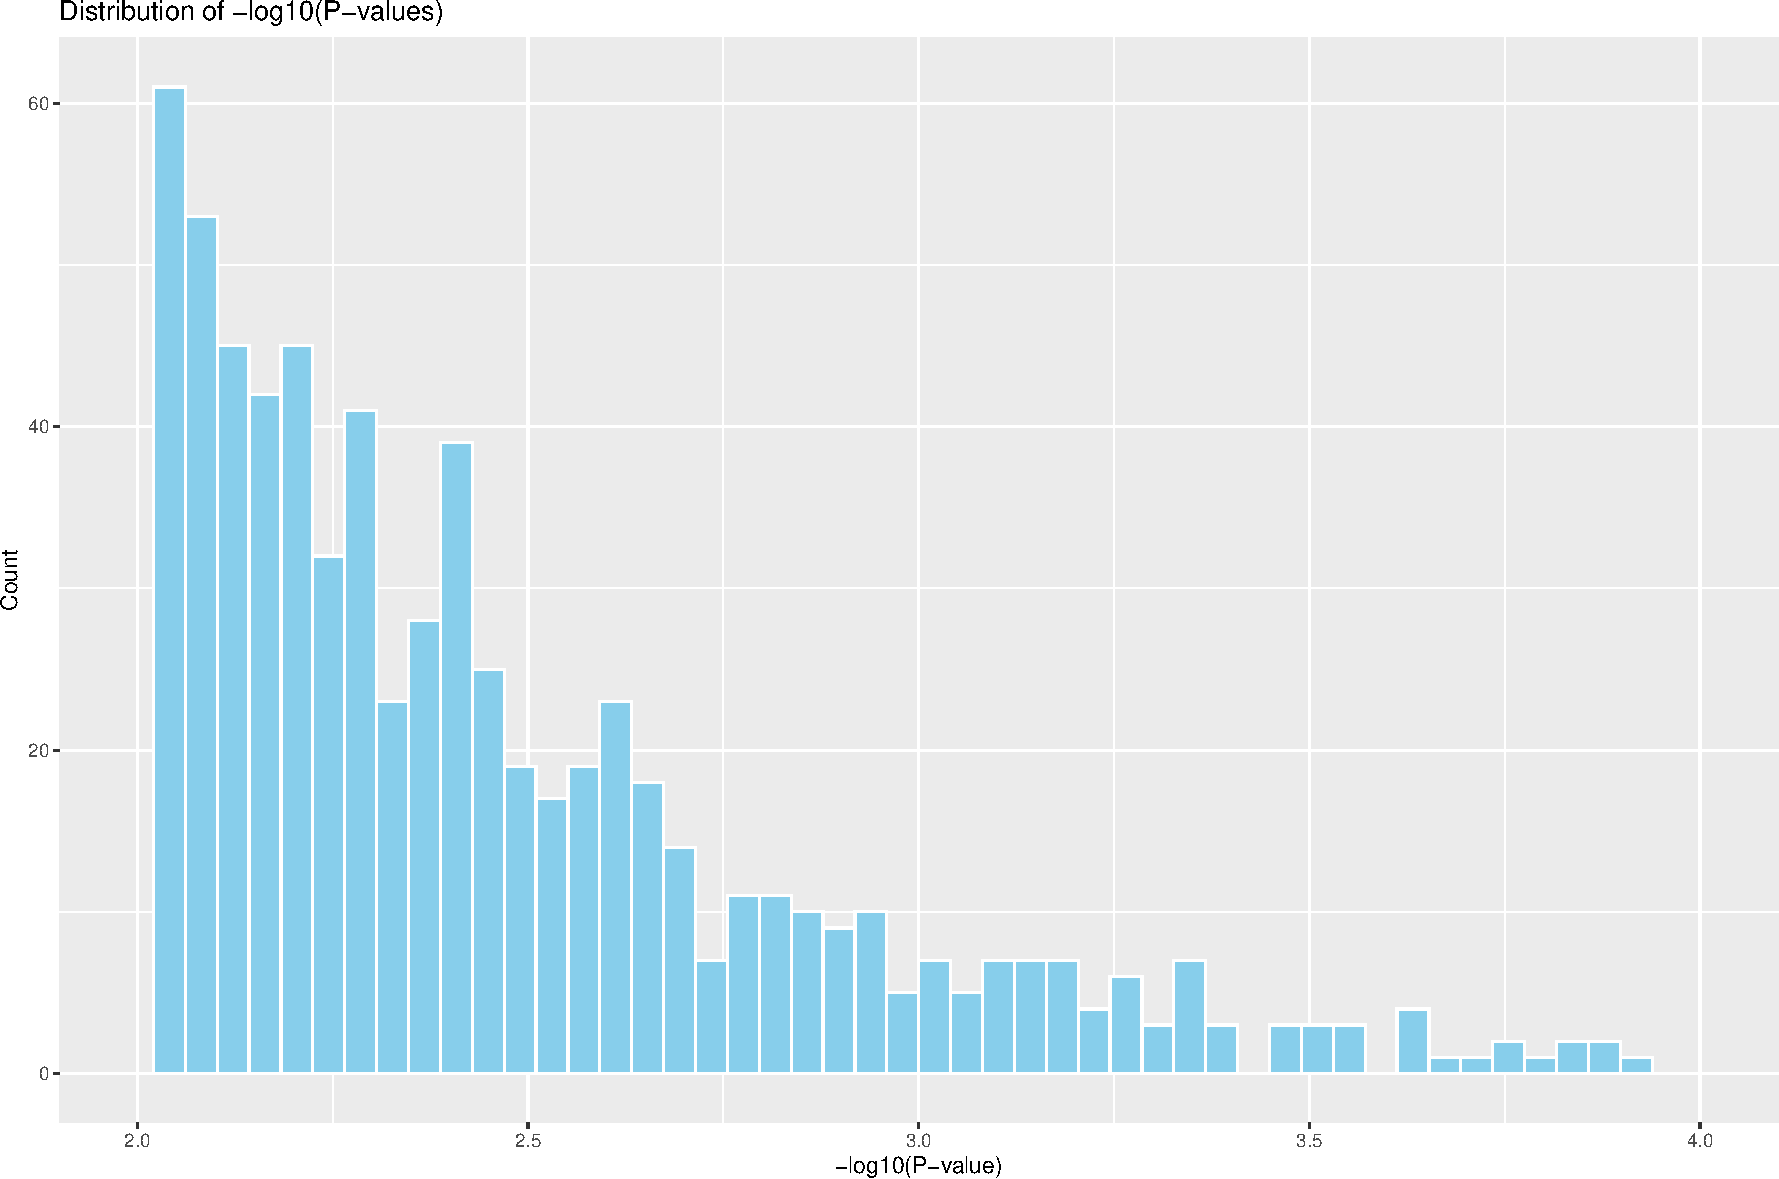
\includegraphics{Arkesh_Das_CMSE_410_Semester_Project_files/figure-latex/normal distribution testing-2.pdf}

\begin{Shaded}
\begin{Highlighting}[]
  \FunctionTok{theme\_minimal}\NormalTok{()}
\end{Highlighting}
\end{Shaded}

\begin{verbatim}
## List of 136
##  $ line                            :List of 6
##   ..$ colour       : chr "black"
##   ..$ linewidth    : num 0.5
##   ..$ linetype     : num 1
##   ..$ lineend      : chr "butt"
##   ..$ arrow        : logi FALSE
##   ..$ inherit.blank: logi TRUE
##   ..- attr(*, "class")= chr [1:2] "element_line" "element"
##  $ rect                            :List of 5
##   ..$ fill         : chr "white"
##   ..$ colour       : chr "black"
##   ..$ linewidth    : num 0.5
##   ..$ linetype     : num 1
##   ..$ inherit.blank: logi TRUE
##   ..- attr(*, "class")= chr [1:2] "element_rect" "element"
##  $ text                            :List of 11
##   ..$ family       : chr ""
##   ..$ face         : chr "plain"
##   ..$ colour       : chr "black"
##   ..$ size         : num 11
##   ..$ hjust        : num 0.5
##   ..$ vjust        : num 0.5
##   ..$ angle        : num 0
##   ..$ lineheight   : num 0.9
##   ..$ margin       : 'margin' num [1:4] 0points 0points 0points 0points
##   .. ..- attr(*, "unit")= int 8
##   ..$ debug        : logi FALSE
##   ..$ inherit.blank: logi TRUE
##   ..- attr(*, "class")= chr [1:2] "element_text" "element"
##  $ title                           : NULL
##  $ aspect.ratio                    : NULL
##  $ axis.title                      : NULL
##  $ axis.title.x                    :List of 11
##   ..$ family       : NULL
##   ..$ face         : NULL
##   ..$ colour       : NULL
##   ..$ size         : NULL
##   ..$ hjust        : NULL
##   ..$ vjust        : num 1
##   ..$ angle        : NULL
##   ..$ lineheight   : NULL
##   ..$ margin       : 'margin' num [1:4] 2.75points 0points 0points 0points
##   .. ..- attr(*, "unit")= int 8
##   ..$ debug        : NULL
##   ..$ inherit.blank: logi TRUE
##   ..- attr(*, "class")= chr [1:2] "element_text" "element"
##  $ axis.title.x.top                :List of 11
##   ..$ family       : NULL
##   ..$ face         : NULL
##   ..$ colour       : NULL
##   ..$ size         : NULL
##   ..$ hjust        : NULL
##   ..$ vjust        : num 0
##   ..$ angle        : NULL
##   ..$ lineheight   : NULL
##   ..$ margin       : 'margin' num [1:4] 0points 0points 2.75points 0points
##   .. ..- attr(*, "unit")= int 8
##   ..$ debug        : NULL
##   ..$ inherit.blank: logi TRUE
##   ..- attr(*, "class")= chr [1:2] "element_text" "element"
##  $ axis.title.x.bottom             : NULL
##  $ axis.title.y                    :List of 11
##   ..$ family       : NULL
##   ..$ face         : NULL
##   ..$ colour       : NULL
##   ..$ size         : NULL
##   ..$ hjust        : NULL
##   ..$ vjust        : num 1
##   ..$ angle        : num 90
##   ..$ lineheight   : NULL
##   ..$ margin       : 'margin' num [1:4] 0points 2.75points 0points 0points
##   .. ..- attr(*, "unit")= int 8
##   ..$ debug        : NULL
##   ..$ inherit.blank: logi TRUE
##   ..- attr(*, "class")= chr [1:2] "element_text" "element"
##  $ axis.title.y.left               : NULL
##  $ axis.title.y.right              :List of 11
##   ..$ family       : NULL
##   ..$ face         : NULL
##   ..$ colour       : NULL
##   ..$ size         : NULL
##   ..$ hjust        : NULL
##   ..$ vjust        : num 1
##   ..$ angle        : num -90
##   ..$ lineheight   : NULL
##   ..$ margin       : 'margin' num [1:4] 0points 0points 0points 2.75points
##   .. ..- attr(*, "unit")= int 8
##   ..$ debug        : NULL
##   ..$ inherit.blank: logi TRUE
##   ..- attr(*, "class")= chr [1:2] "element_text" "element"
##  $ axis.text                       :List of 11
##   ..$ family       : NULL
##   ..$ face         : NULL
##   ..$ colour       : chr "grey30"
##   ..$ size         : 'rel' num 0.8
##   ..$ hjust        : NULL
##   ..$ vjust        : NULL
##   ..$ angle        : NULL
##   ..$ lineheight   : NULL
##   ..$ margin       : NULL
##   ..$ debug        : NULL
##   ..$ inherit.blank: logi TRUE
##   ..- attr(*, "class")= chr [1:2] "element_text" "element"
##  $ axis.text.x                     :List of 11
##   ..$ family       : NULL
##   ..$ face         : NULL
##   ..$ colour       : NULL
##   ..$ size         : NULL
##   ..$ hjust        : NULL
##   ..$ vjust        : num 1
##   ..$ angle        : NULL
##   ..$ lineheight   : NULL
##   ..$ margin       : 'margin' num [1:4] 2.2points 0points 0points 0points
##   .. ..- attr(*, "unit")= int 8
##   ..$ debug        : NULL
##   ..$ inherit.blank: logi TRUE
##   ..- attr(*, "class")= chr [1:2] "element_text" "element"
##  $ axis.text.x.top                 :List of 11
##   ..$ family       : NULL
##   ..$ face         : NULL
##   ..$ colour       : NULL
##   ..$ size         : NULL
##   ..$ hjust        : NULL
##   ..$ vjust        : num 0
##   ..$ angle        : NULL
##   ..$ lineheight   : NULL
##   ..$ margin       : 'margin' num [1:4] 0points 0points 2.2points 0points
##   .. ..- attr(*, "unit")= int 8
##   ..$ debug        : NULL
##   ..$ inherit.blank: logi TRUE
##   ..- attr(*, "class")= chr [1:2] "element_text" "element"
##  $ axis.text.x.bottom              : NULL
##  $ axis.text.y                     :List of 11
##   ..$ family       : NULL
##   ..$ face         : NULL
##   ..$ colour       : NULL
##   ..$ size         : NULL
##   ..$ hjust        : num 1
##   ..$ vjust        : NULL
##   ..$ angle        : NULL
##   ..$ lineheight   : NULL
##   ..$ margin       : 'margin' num [1:4] 0points 2.2points 0points 0points
##   .. ..- attr(*, "unit")= int 8
##   ..$ debug        : NULL
##   ..$ inherit.blank: logi TRUE
##   ..- attr(*, "class")= chr [1:2] "element_text" "element"
##  $ axis.text.y.left                : NULL
##  $ axis.text.y.right               :List of 11
##   ..$ family       : NULL
##   ..$ face         : NULL
##   ..$ colour       : NULL
##   ..$ size         : NULL
##   ..$ hjust        : num 0
##   ..$ vjust        : NULL
##   ..$ angle        : NULL
##   ..$ lineheight   : NULL
##   ..$ margin       : 'margin' num [1:4] 0points 0points 0points 2.2points
##   .. ..- attr(*, "unit")= int 8
##   ..$ debug        : NULL
##   ..$ inherit.blank: logi TRUE
##   ..- attr(*, "class")= chr [1:2] "element_text" "element"
##  $ axis.text.theta                 : NULL
##  $ axis.text.r                     :List of 11
##   ..$ family       : NULL
##   ..$ face         : NULL
##   ..$ colour       : NULL
##   ..$ size         : NULL
##   ..$ hjust        : num 0.5
##   ..$ vjust        : NULL
##   ..$ angle        : NULL
##   ..$ lineheight   : NULL
##   ..$ margin       : 'margin' num [1:4] 0points 2.2points 0points 2.2points
##   .. ..- attr(*, "unit")= int 8
##   ..$ debug        : NULL
##   ..$ inherit.blank: logi TRUE
##   ..- attr(*, "class")= chr [1:2] "element_text" "element"
##  $ axis.ticks                      : list()
##   ..- attr(*, "class")= chr [1:2] "element_blank" "element"
##  $ axis.ticks.x                    : NULL
##  $ axis.ticks.x.top                : NULL
##  $ axis.ticks.x.bottom             : NULL
##  $ axis.ticks.y                    : NULL
##  $ axis.ticks.y.left               : NULL
##  $ axis.ticks.y.right              : NULL
##  $ axis.ticks.theta                : NULL
##  $ axis.ticks.r                    : NULL
##  $ axis.minor.ticks.x.top          : NULL
##  $ axis.minor.ticks.x.bottom       : NULL
##  $ axis.minor.ticks.y.left         : NULL
##  $ axis.minor.ticks.y.right        : NULL
##  $ axis.minor.ticks.theta          : NULL
##  $ axis.minor.ticks.r              : NULL
##  $ axis.ticks.length               : 'simpleUnit' num 2.75points
##   ..- attr(*, "unit")= int 8
##  $ axis.ticks.length.x             : NULL
##  $ axis.ticks.length.x.top         : NULL
##  $ axis.ticks.length.x.bottom      : NULL
##  $ axis.ticks.length.y             : NULL
##  $ axis.ticks.length.y.left        : NULL
##  $ axis.ticks.length.y.right       : NULL
##  $ axis.ticks.length.theta         : NULL
##  $ axis.ticks.length.r             : NULL
##  $ axis.minor.ticks.length         : 'rel' num 0.75
##  $ axis.minor.ticks.length.x       : NULL
##  $ axis.minor.ticks.length.x.top   : NULL
##  $ axis.minor.ticks.length.x.bottom: NULL
##  $ axis.minor.ticks.length.y       : NULL
##  $ axis.minor.ticks.length.y.left  : NULL
##  $ axis.minor.ticks.length.y.right : NULL
##  $ axis.minor.ticks.length.theta   : NULL
##  $ axis.minor.ticks.length.r       : NULL
##  $ axis.line                       : list()
##   ..- attr(*, "class")= chr [1:2] "element_blank" "element"
##  $ axis.line.x                     : NULL
##  $ axis.line.x.top                 : NULL
##  $ axis.line.x.bottom              : NULL
##  $ axis.line.y                     : NULL
##  $ axis.line.y.left                : NULL
##  $ axis.line.y.right               : NULL
##  $ axis.line.theta                 : NULL
##  $ axis.line.r                     : NULL
##  $ legend.background               : list()
##   ..- attr(*, "class")= chr [1:2] "element_blank" "element"
##  $ legend.margin                   : 'margin' num [1:4] 5.5points 5.5points 5.5points 5.5points
##   ..- attr(*, "unit")= int 8
##  $ legend.spacing                  : 'simpleUnit' num 11points
##   ..- attr(*, "unit")= int 8
##  $ legend.spacing.x                : NULL
##  $ legend.spacing.y                : NULL
##  $ legend.key                      : list()
##   ..- attr(*, "class")= chr [1:2] "element_blank" "element"
##  $ legend.key.size                 : 'simpleUnit' num 1.2lines
##   ..- attr(*, "unit")= int 3
##  $ legend.key.height               : NULL
##  $ legend.key.width                : NULL
##  $ legend.key.spacing              : 'simpleUnit' num 5.5points
##   ..- attr(*, "unit")= int 8
##  $ legend.key.spacing.x            : NULL
##  $ legend.key.spacing.y            : NULL
##  $ legend.frame                    : NULL
##  $ legend.ticks                    : NULL
##  $ legend.ticks.length             : 'rel' num 0.2
##  $ legend.axis.line                : NULL
##  $ legend.text                     :List of 11
##   ..$ family       : NULL
##   ..$ face         : NULL
##   ..$ colour       : NULL
##   ..$ size         : 'rel' num 0.8
##   ..$ hjust        : NULL
##   ..$ vjust        : NULL
##   ..$ angle        : NULL
##   ..$ lineheight   : NULL
##   ..$ margin       : NULL
##   ..$ debug        : NULL
##   ..$ inherit.blank: logi TRUE
##   ..- attr(*, "class")= chr [1:2] "element_text" "element"
##  $ legend.text.position            : NULL
##  $ legend.title                    :List of 11
##   ..$ family       : NULL
##   ..$ face         : NULL
##   ..$ colour       : NULL
##   ..$ size         : NULL
##   ..$ hjust        : num 0
##   ..$ vjust        : NULL
##   ..$ angle        : NULL
##   ..$ lineheight   : NULL
##   ..$ margin       : NULL
##   ..$ debug        : NULL
##   ..$ inherit.blank: logi TRUE
##   ..- attr(*, "class")= chr [1:2] "element_text" "element"
##  $ legend.title.position           : NULL
##  $ legend.position                 : chr "right"
##  $ legend.position.inside          : NULL
##  $ legend.direction                : NULL
##  $ legend.byrow                    : NULL
##  $ legend.justification            : chr "center"
##  $ legend.justification.top        : NULL
##  $ legend.justification.bottom     : NULL
##  $ legend.justification.left       : NULL
##  $ legend.justification.right      : NULL
##  $ legend.justification.inside     : NULL
##  $ legend.location                 : NULL
##  $ legend.box                      : NULL
##  $ legend.box.just                 : NULL
##  $ legend.box.margin               : 'margin' num [1:4] 0cm 0cm 0cm 0cm
##   ..- attr(*, "unit")= int 1
##  $ legend.box.background           : list()
##   ..- attr(*, "class")= chr [1:2] "element_blank" "element"
##  $ legend.box.spacing              : 'simpleUnit' num 11points
##   ..- attr(*, "unit")= int 8
##   [list output truncated]
##  - attr(*, "class")= chr [1:2] "theme" "gg"
##  - attr(*, "complete")= logi TRUE
##  - attr(*, "validate")= logi TRUE
\end{verbatim}

\begin{Shaded}
\begin{Highlighting}[]
\CommentTok{\#To create figure in slide deck}
\NormalTok{x }\OtherTok{\textless{}{-}} \FunctionTok{seq}\NormalTok{(}\SpecialCharTok{{-}}\DecValTok{4}\NormalTok{, }\DecValTok{4}\NormalTok{, }\AttributeTok{length.out =} \DecValTok{1000}\NormalTok{)}
\NormalTok{y }\OtherTok{\textless{}{-}} \FunctionTok{dnorm}\NormalTok{(x)}

\NormalTok{df\_norm }\OtherTok{\textless{}{-}} \FunctionTok{data.frame}\NormalTok{(}\AttributeTok{x =}\NormalTok{ x, }\AttributeTok{y =}\NormalTok{ y)}

\NormalTok{z\_cutoff }\OtherTok{\textless{}{-}} \FunctionTok{qnorm}\NormalTok{(}\FloatTok{0.95}\NormalTok{)  }

\NormalTok{shade\_df }\OtherTok{\textless{}{-}} \FunctionTok{subset}\NormalTok{(df\_norm, x }\SpecialCharTok{\textgreater{}}\NormalTok{ z\_cutoff)}


\FunctionTok{ggplot}\NormalTok{(df\_norm, }\FunctionTok{aes}\NormalTok{(x, y)) }\SpecialCharTok{+}
  \FunctionTok{geom\_line}\NormalTok{(}\AttributeTok{color =} \StringTok{"black"}\NormalTok{, }\AttributeTok{size =} \DecValTok{1}\NormalTok{) }\SpecialCharTok{+}  \CommentTok{\# Normal curve}
  \FunctionTok{geom\_area}\NormalTok{(}\AttributeTok{data =}\NormalTok{ shade\_df, }\FunctionTok{aes}\NormalTok{(x, y), }\AttributeTok{fill =} \StringTok{"skyblue"}\NormalTok{, }\AttributeTok{alpha =} \FloatTok{0.6}\NormalTok{) }\SpecialCharTok{+} 
  \FunctionTok{geom\_vline}\NormalTok{(}\AttributeTok{xintercept =}\NormalTok{ z\_cutoff, }\AttributeTok{color =} \StringTok{"red"}\NormalTok{, }\AttributeTok{linetype =} \StringTok{"dashed"}\NormalTok{, }\AttributeTok{size =} \DecValTok{1}\NormalTok{) }\SpecialCharTok{+}  
  \FunctionTok{labs}\NormalTok{(}
    \AttributeTok{title =} \StringTok{"Standard Normal Distribution with One{-}Sided p = 0.05 Cutoff"}\NormalTok{,}
    \AttributeTok{x =} \StringTok{"Z{-}score"}\NormalTok{,}
    \AttributeTok{y =} \StringTok{"Density"}
\NormalTok{  ) }\SpecialCharTok{+}
  \FunctionTok{theme\_minimal}\NormalTok{()}
\end{Highlighting}
\end{Shaded}

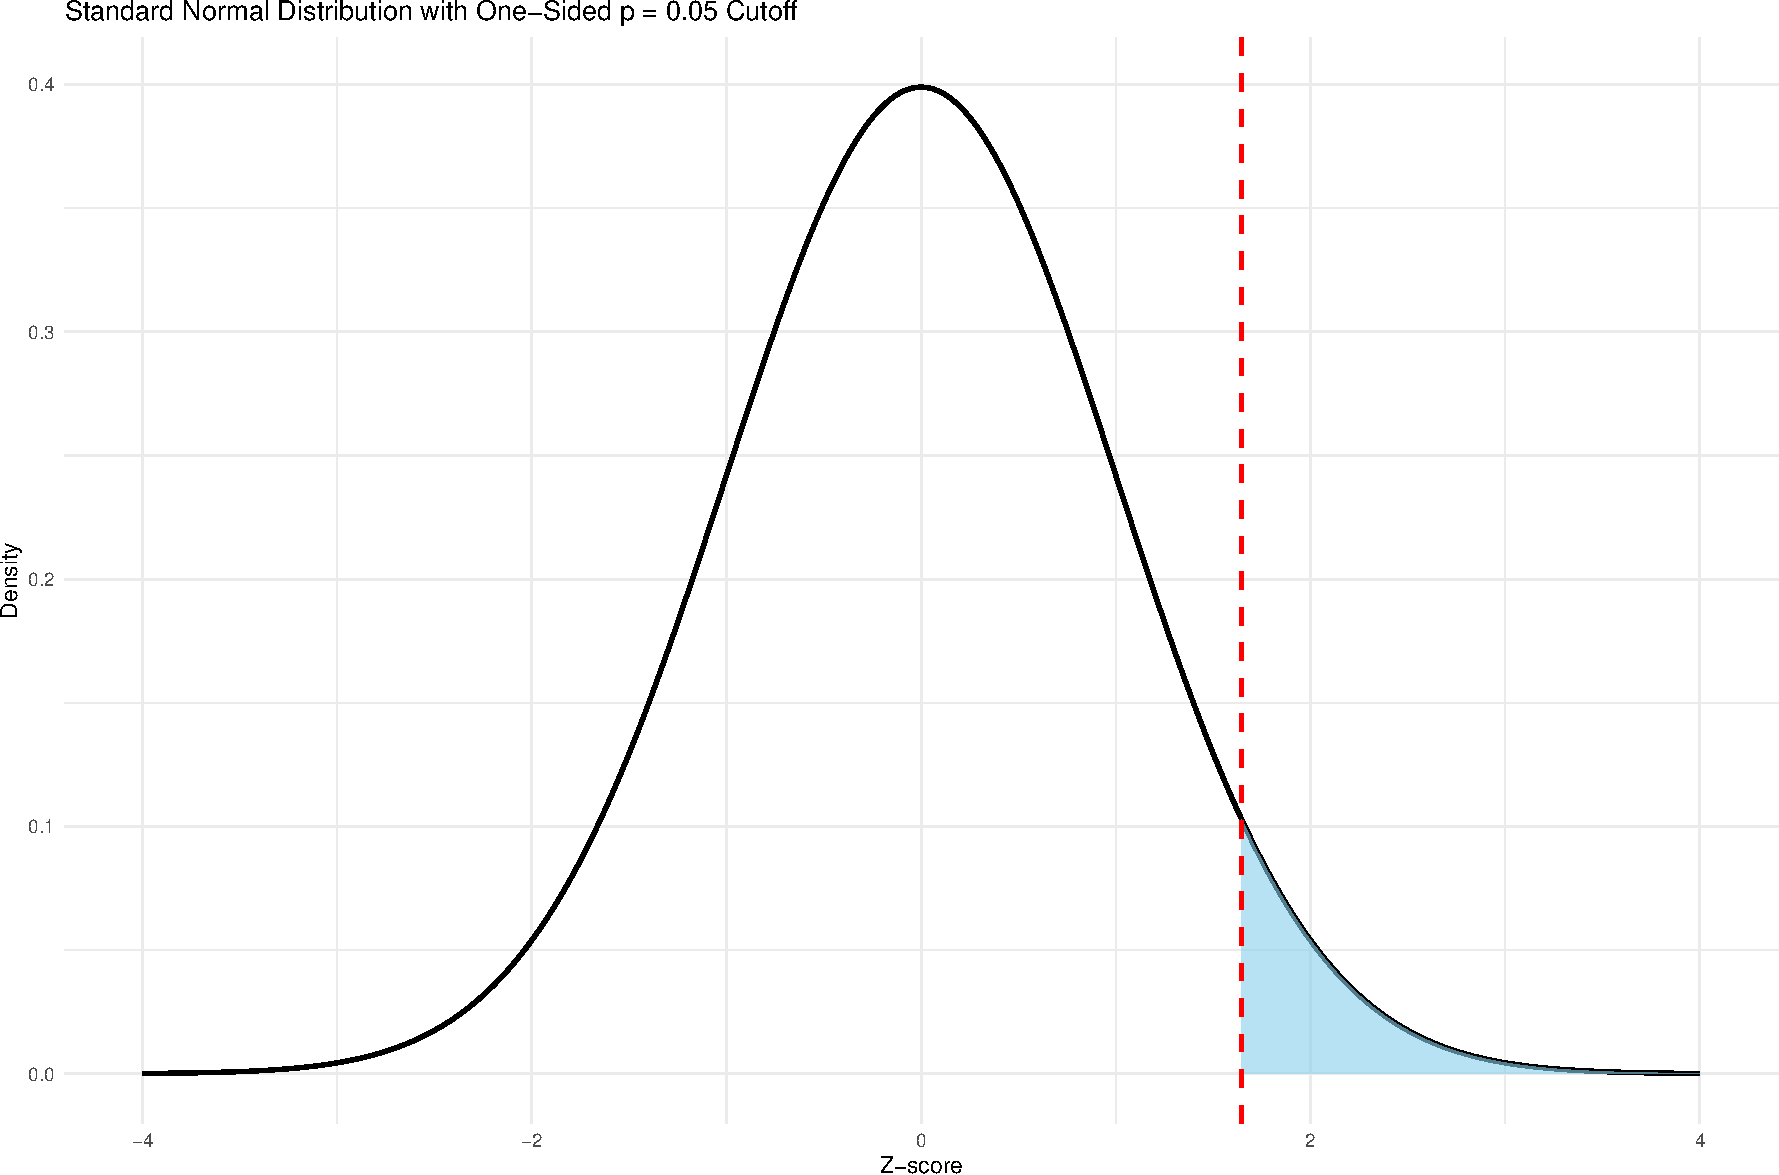
\includegraphics{Arkesh_Das_CMSE_410_Semester_Project_files/figure-latex/normal dist curve-1.pdf}

\section{References}\label{references}

{[}1{]}
\url{https://www.milieuinterieur.fr/en/about-us/the-milieu-interieur/}

{[}2{]}Scepanovic, P., Alanio, C., Hammer, C., et al.~(2018). Human
genetic variants and age are the strongest predictors of humoral immune
responses to common pathogens and vaccines. Genome Medicine, 10, 59.
\url{https://doi.org/10.1186/s13073-018-0568-8}

{[}3{]}
\url{https://www.rdocumentation.org/packages/qqman/versions/0.1.2/topics/manhattan}

{[}4{]}
\url{https://search.r-project.org/CRAN/refmans/mutoss/html/multiple.down.html}

{[}5{]} Benjamini, Y., Krieger, A. M., \& Yekutieli, D. (2006). Adaptive
Linear Step-up Procedures That Control the False Discovery Rate.
Biometrika, 93(3), 491--507.
\url{https://doi.org/10.1093/biomet/93.3.491}

{[}6{]} Storey JD, Tibshirani R. Statistical significance for genomewide
studies. Proc Natl Acad Sci U S A. 2003 Aug 5;100(16):9440-5. doi:
10.1073/pnas.1530509100. Epub 2003 Jul 25. PMID: 12883005; PMCID:
PMC170937.

{[}7{]}
\url{https://www.rdocumentation.org/packages/qvalue/versions/2.4.2/topics/qvalue}

{[}8{]} \url{https://www.ncbi.nlm.nih.gov/gdv/}

{[}9{]} Arai S, Miyazaki T. Impaired maturation of myeloid progenitors
in mice lacking novel Polycomb group protein MBT-1. EMBO J. 2005 May
18;24(10):1863-73. doi: 10.1038/sj.emboj.7600654

\end{document}
